\documentclass[journal,twocolumn]{IEEEtran}

%\usepackage[ansinew]{inputenc}
\usepackage{graphicx}
\usepackage{psfrag}
\usepackage{stfloats}
%\usepackage[spanish]{babel}
\usepackage{epsfig}
\usepackage{pifont}
\usepackage{amssymb}
\usepackage{fixltx2e}
\usepackage{amsmath}
\usepackage{rotate}
\usepackage{anysize}
%\usepackage{rotating}
%\usepackage{fancybox}
\usepackage{float}
\usepackage{fancybox}
\usepackage{subfig}

\newcommand{\pig}[1]{\mbox{\boldmath ${#1}$}	}

\newtheorem{Theod}{{\bf Definici\'on}}

\setlength{\oddsidemargin}{5mm}
\setlength{\evensidemargin}{5mm}
\setlength{\topmargin}{4mm}
\setlength{\textwidth}{15cm}
\setlength{\columnsep}{5mm}
\setlength{\textheight}{24cm}

\begin{document}

\title{A thorough explanation of the  double bounded polynomial homotopy applied to non-linear circuit simulation 
\newline\newline
Une explication d\'etaill\'ee de l'homotopie polyn\^omiale doublement limit\'ee appliqu\'ee \`a la simulation des circuits non-linéaire
}

\author{H\'ector V\'azquez-Leal$^1$\thanks{H.
V\'azquez, R. Casta\~neda and D. Pereyra  are with the Universidad Veracruza, Facultad de Instrumentaci\'on Electr\'onica y Ciencias Atmosf\'ericas, Xalapa, Veracruz, Mexico. E-mail:
[hvazquez]@uv.mx}, Luis Hern\'andez-Mart\'{\i}nez$^2$\thanks{L.
Hern\'andez , A. Sarmiento are with the Electronics Department, CAD Group,
National Institute for Astrophysics Optics and Electronics
(INAOE), P.O. Box 51, 72000, Puebla, Pue., Mexico. E-mail:
[luish, jarocho]@inaoep.mx} \\ Arturo Sarmiento-Reyes$^2$, Roberto Casta\~neda-Sheissa$^1$ and Domitilo Pereyra-D{\'i}az$^1$}

%\author{\authorblockN{H\'ector V\'azquez-Leal, Roberto Casta\~neda\\ and Domitilo Pereyra-D{\'i}5az} 
%\authorblockA{Universidad Veracruzana\\
%Facultad de Instrumentaci\'on Electr\'onica\\
%Xalapa, Veracruz, M\'exico\\
%Email: hvazquez@uv.mx\\}
%\and
%\authorblockN{Luis Hern\'andez-Mart\'{\i}nez\\Arturo Sarmiento-Reyes}
%\authorblockA{INAOE\\
%Departamento de Electr\'onica\\
%Puebla, Puebla, M\'exico\\
%Email: luish@inaope.mx}
%}

\maketitle

\begin{abstract}

This work shows a new double bounded Homotopy based on polynomial formulation. It presents a bounding between two solution lines and a symmetry axis,which allows to establish a stop criterion for the simulation. Besides, the initial and final points for the new double bounded Homotopy may be established in an arbitrary manner. Mathematical properties will be introduced for this new Homotopy, besides, some mathematical and circuital examples will be discussed.

%\end{abstract}

\vspace{6mm}
%\begin{abstract}

{\bfseries\textit{R\'esum\'e}--- } Ce travail montre une nouvelle homotopie doublement limit\'ee, bas\'ee sur une formulation polynomiale. Il pr\'esente une limite entre deux lignes de solution, et il pr\'esente aussi un axe de sym\'etrie; tout ça permet d'\'etablir un crit\`ere d'arr\^et pour la simulation. D'ailleurs, les points initial et final pour la nouvelle homotopie doublement limit\'ee, peuvent \^etre \'etablie de mani\`ere arbitraire. Les propri\'et\'es math\'ematiques seront mises en place pour cette nouvelle homotopie, et en plus, quelques exemples math\'ematiques et exemples de circuits seront discut\'es.
\end{abstract}

\begin{keywords}
Homotopy continuation methods, DC analysis, path following techniques.
\end{keywords}

\section{Introduction}

The research and development in the electronics industry has proven being very important activities on developed countries, causing a big impact in their economies, creating better conditions for development of their population and offering conditions to improve their performance on daily duties. The electronics industry, as demanding as competitive, constantly is pushing the physical area of circuits to the very limits of human knowledge. As a consequence, the rapid growth of integration levels for integrated circuits (IC). In fact, the 2 billion transistor mark was reached in 2008. Also, the noticeable advance in technologies at nanometer scales has affected other knowledge areas like device modeling, simulation techniques for integrated circuits, materials science, among others. Therefore, it is necessary to develop new and better simulation techniques for the purpose of simulate the behavior of circuits that have become more complex. Specifically, the Homotopy has a direct impact in IC simulation tools and, in general, in whichever science area where the phenomenon can be modeled by non-linear equations system.

Integrated circuits could have more than one operating point or DC solution, one way to resolve such points is by the use of Homotopy methods \cite{cont_chu1}. The problem to find solutions in DC is important because this analysis serves as initial point for the rest of analysis performed routinely during the circuit design (for instance, small signal analysis)\cite{homo_ogrodzki}. This analysis consists in finding solutions for non-linear algebraic equations system (NAEs) originating from integrated circuits \cite{Schwa_book}. These NAEs become complex because the accelerated increase on the number of transistors by ICs and the increase of complexity of models (as the result of reducing the physical dimensions of the components) causing two situations: existence for multiple unexpected operating points, and lack of convergence to the operating point in Newton's method.

The Newton-Raphson method (NR) is employed in many circuit simulators for integrated circuit. The widespread use of the NR method is its quadratic convergence rate \cite{homo_ogrodzki,cont_quasi} which minimizes computation times in simulations. Nevertheless, the NR method has certain convergence problems \cite{cont_quasi,Schwa_book} like: oscillation and divergence. Convergence problem becomes apparent in electronics when non-linear equation systems ($f(x)$) from elaborated systems are resolved, and these complicated systems mix analog and digital blocks. Therefore, the need to develop backup methods or replace the NR method.

Electronic circuit designers usually deal with convergence failures using the NR method, thus as  last resource, some parameters in the numerical engine of the simulator are modified hoping to reach convergence. This situation breaks design schedules. Also, justifies the use of alternate methods to NR like Homotopy to locate the operating point. Nevertheless, there are many reasons for using Homotopy like occurrence of more than one operating point. That is, unlike the NR method, Homotopy is capable to locate multiple operating points. This is very important because it may occur that a designer provides one operating point as valid in DC (found by the NR method) but other operating point, one of many that the circuit may contain, is physically present in the already fabricated circuit. This may translate into the circuit  malfunctioning  with costly consequences for a company.

This situation has prompted investigations to develop new methods capable to solve non-linear equation systems in an efficient and accurate process.

Homotopy methods \cite{BHLHOM,homo_ushida1,homo_green2,homo_DWolfMulti,homo_ArtificialP} are valuable tools for simulation, presented as an alternate method to the NR method. However, Homotopy methods have two problems: stop criterion and computing time.

\section{Double bounded Homotopy}

Considering the existence of two solution lines \cite{homo_iscas05,homo_iberchip03}, one at $\lambda=a$ and the other at $\lambda=b$; so the Homotopy formulation is:

\begin{equation}
\pig{H}(\pig{f}(\pig{x}),\lambda ) =\pig{0}
\label{H2M}
\end{equation}

where $f(x)$ is the equilibrium equation, $\lambda$ is the Homotopy variable, and $\pig{H}^{-1}(\pig{0})$ are the family of solutions that outlines the Homotopy patch, such that:

\begin{itemize}
\item For $\lambda=0.5(a+b)$ solution for $H^{-1}(0)$ is known or simple to calculate computationally. This point is known as initial point in Homotopy ($\lambda_i$).
\item For $\lambda=a$, $\pig{H}(\pig{f}(\pig{x}),\pig{a} )=\pig{f}(\pig{x})$. It means that at $\lambda=a$ all solutions for $\pig{f}(\pig{x})$ are located.
\item For $\lambda=b$, $\pig{H}(\pig{f}(\pig{x}),\pig{b} )=\pig{f}(\pig{x})$. Means that at $\lambda=b$ all solutions for $\pig{f}(\pig{x})$ are located.
\item The path for $\pig{H}^{-1}(\pig{0})$  is a continuous function for $\lambda$ in the range of $a \leq \lambda \leq b $. 
\end{itemize}

\section{Double bounded polynomial Homotopy}

The double bounded polynomial Homotopy (DBP) is defined by the following equation:

\begin{equation}
{\tiny
\begin{array}{l}
\pig{H}(\pig{f}(\pig{x}),\lambda )=Q(x-x_i)(x-x_f) -C(\lambda-a/2)^2 \pig{f}(\pig{x})^2
\end{array}}
\label{homotopiaP}
\end{equation}


where $Q=\lambda(\lambda-a)$, $a$ is a constant that represents the separation between solution lines, $x_i$ is the initial point, $x_f$ the final point, and $C$ an arbitrary constant.

Based on the preceding, Homotopy can be expressed in general way as:

{\tiny
\begin{displaymath}
\pig{H}(\pig{f}(\pig{x}),\lambda ) = \left\{\begin{array}{rl}
f(x^*)=0 & \textrm{para $\lambda=0$ y $x=x^*$}\\
(x-x_i)(x-x_f)=0 & \textrm{para $\lambda=a/2$}\\
f(x^*)=0 & \textrm{para $\lambda=a$ y $x=x^*$}
\end{array}\right.
\end{displaymath}
}
where $x^*$ is any solution for the equilibrium equation $f(x)$, $x_i$ in the initial point, while $x_f$ is the final point for outline the path.

This Homotopy has two solution lines ($\lambda=0$ y $\lambda=a$). Squaring function $f(x)$ originates an even number of solutions (or operating points) resulting in the bounding of it and closes the Homotopy path within the middle region. Figure \ref{halftrack} shows how the Homotopy path initiates at $A=(x_i,a/2)$ on the symmetry axis, finds two roots (in region $\lambda_2(x)$) and, finally, ends when a new crossing the symmetry axis at $B=(x_f,a/2)$ meaning that the tracing of a symmetrical branch is completed fulfilling the stop criterion.

\begin{figure}[hbtp]
\psfrag{o}{$\lambda$}
\centering
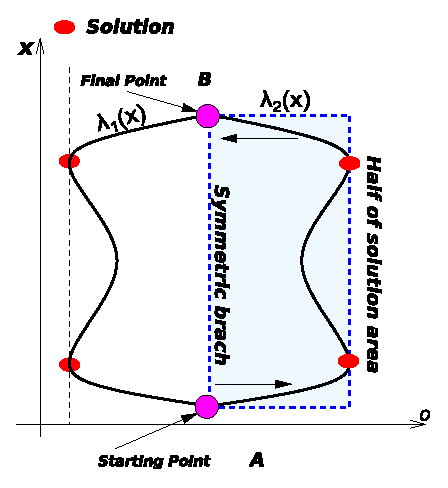
\includegraphics[scale=0.7]{nh3figs/dbh2.eps}
\caption{Stop criterion.}
\label{halftrack}
\end{figure}

Properties of this new Homotopy are presented in the following sub-sections:

\subsection{Symmetrical branches}

Symmetrical branches shown in figure \ref{halftrack} can be obtained solving for $\lambda$ equation \ref{homotopiaP}. The result is two symmetrical branches (ecuaciones \ref{SB1} y \ref{SB2}), where each symmetrical branch $\lambda_1(x)$ and $\lambda_2(x)$is tied to a different solution line $\lambda=0$ and $\lambda=a$, respectively. Given that $\lambda_1(x)$ and $\lambda_2(x)$ are connected and symmetrical, it is just necessary to trace only one of them to obtain the complete path and finish the simulation. $\lambda_2(x)$ is chosen as the path to trace, it touches tangentially solution line $\lambda=a$.

\begin{equation}
\lambda_1(x)= {\frac {\left( \sqrt {1-{\frac {C \left( f \left( x \right)  \right) ^{2
}}{ \left( x-x_i \right)  \left( x-x_f \right) }}}-1
 \right) a}{2\sqrt {1-{\frac {C \left( f \left( x \right) 
 \right) ^{2}}{ \left( x-x_i \right)  \left( x-x_f
 \right) }}}}}
\label{SB1}
\end{equation}

\begin{equation}
\lambda_2(x)= {\frac {\left( \sqrt {1-{\frac {C \left( f \left( x \right)  \right) ^{2
}}{ \left( x-x_i \right)  \left( x-x_f \right) }}}+1
 \right) a}{2\sqrt {1-{\frac {C \left( f \left( x \right) 
 \right) ^{2}}{ \left( x-x_i \right)  \left( x-x_f
 \right) }}}}}
\label{SB2}
\end{equation}

To demonstrate that $\lambda_1(x)$ is linked to the solution line $\lambda=0$, the following limit is calculated:

\begin{equation}
 \displaystyle\lim_{f(x) \to{0}}{\lambda_1(x)}=0 
 \label{demos1x}
\end{equation}

the equilibrium equation $f(x)$ tends to zero when $x$ tends to solution $x^*$, as shown in the following limit calculation:

\begin{equation}
 \displaystyle\lim_{x \to{x^*}}{f(x)}=0 
 \label{demos1x2}
\end{equation}

Now, to demonstrate that $\lambda_2(x)$ is linked to the solution line $\lambda=a$, the following limit is calculated:

\begin{equation}
 \displaystyle\lim_{f(x) \to{0}}{\lambda_2(x)}=a 
 \label{demos2x}
\end{equation}

%where the equilibrium equation $f(x)$ tends to "$a$" when $x$ tends to solution $x^*$, as shown in the following limit calculation:

%\begin{equation}
% \displaystyle\lim_{x \to{x^*}}{f(x)}=a 
% \label{demos1x3}
%\end{equation}

\subsection{Symmetry axis}

Symmetry axis is an important property in the double bounded Homotopy. In the particular case of the double bounded polynomial Homotopy the symmetry axis is:

\begin{equation}
\lambda_{sym}= {a \over 2}
\label{sym}
\end{equation}

This symmetry axis belongs to the symmetry relationship between $\lambda_1(x)$ and $\lambda_2(x)$.

As shown in figure \ref{simetria}, the following relationship must be satisfied:

\begin{displaymath}
\lambda_2(x)-\lambda_{sym}=\lambda_{sym} -\lambda_1(x)
\end{displaymath}

Replacing the value for $\lambda_{sym}$ it is obtained that:

\begin{displaymath}
\lambda_2(x)-0.5a=0.5a-\lambda_1(x)
\end{displaymath}

Reordering terms:

\begin{displaymath}
\begin{array}{l}
\lambda_2(x)+\lambda_1(x)=a
\end{array}
\end{displaymath}

Substituting values for $\lambda_1(x)$ and $\lambda_2(x)$ by their respective functions, the following relationship is obtained:

\begin{displaymath}
\begin{array}{l}
a=a
\end{array}
\end{displaymath}

Removing terms results:

\begin{displaymath}
\begin{array}{c}
0=0
\end{array}
\end{displaymath}

Proofing this equality shows that the Homotopy path is symmetrical around the symmetry axis.

{
\tiny
\begin{figure}[hbtp]
\psfrag{o}{\tiny $\lambda$}
\psfrag{o1}{\tiny $\lambda_2(x)$}
\psfrag{o2}{\tiny $\lambda_1(x)$}
\psfrag{o3}{\tiny $\lambda_2(x)-\lambda_{sym}$}
\psfrag{o4}{\tiny $\lambda_{sym}-\lambda_1(x)$}
\centering
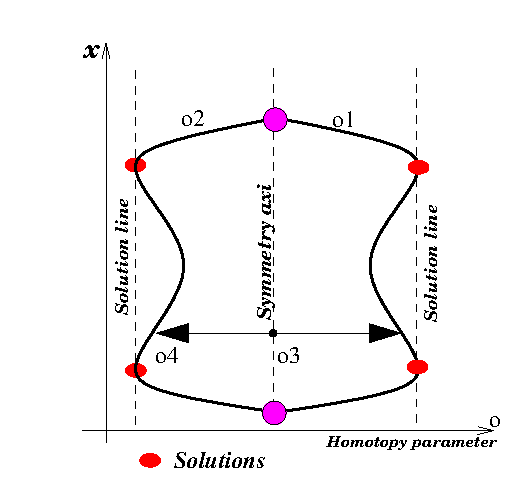
\includegraphics[width=7cm]{nh3figs/simetria.eps}
\caption{The homotopy path have symmetry}
\label{simetria}
\end{figure}
}

\subsection{Initial point and final point}

The point where the Homotopy path starts lays right on the symmetry axis, meaning that $\lambda_i=0.5a$. Therefore, replacing $\lambda_i$ in equation \ref{homotopiaP} the term that contains the equilibrium equation $f(x)$ is canceled, resulting:

\begin{displaymath}
\begin{array}{r}
\pig{H}(\pig{f}(\pig{x}),\lambda_i )=(x-x_i)(x-x_f)=0  \\
\end{array}
\end{displaymath}

So the initial ($x_i$) and final ($x_f$) points are chosen arbitrarily.

In order to prove that $\lambda_1(x)$ crosses the symmetry axis at $x_i$ and $x_f$, the following limits are calculated:

\begin{equation}
\begin{array}{r}
 \displaystyle\lim_{x \to{x_i}}{\lambda_1(x)}=0.5a \\
  \displaystyle\lim_{x \to{x_f}}{\lambda_1(x)}=0.5a 
 \end{array}
 \label{simetriax2}
\end{equation}

To demonstrate that $\lambda_2(x)$ crosses the symmetry axis at $x_i$ and $x_f$, the following limits are calculated:

\begin{equation}
\begin{array}{r}
 \displaystyle\lim_{x \to{x_i}}{\lambda_2(x)}=0.5a \\
  \displaystyle\lim_{x \to{x_f}}{\lambda_2(x)}=0.5a 
 \end{array}
 \label{simetriax3}
\end{equation}

Therefore, when $x$ tends to the value of initial point $x_i$ or final point $x_f$, the Homotopy parameter $\lambda$ tends to the symmetry axis at $\lambda=0.5a$.

\subsection{Circuital rendering}

Circuital rendering for the double bounded Homotopy can be derived solving $f(x)$ from the Homotopy expression in equation \ref{homotopiaP}. From former equation can be deduced that non-linear current sources are present ($K_1$, $\hdots$ ,$K_n$) connected to every node of the circuit, where $n$ is the number of nodes and $l$ the number of constant voltage sources ($E$).

\begin{equation}
I_{K_m}={\lambda(\lambda-a)(V_{m}-V_{i})(V_{m}-V_{f}) \over (\lambda-a/2)^2}
\label{Ikn}
\end{equation}

where $m=[1,n]$, $V_{xk}$ are nodal voltages for the circuit, $V_{{xk}_i}$ and $V_{{xk}_f}$ are constants related to initial and final points for each variable $V_{xk}$ of the Homotopy. Again, from equation (2), it can be deduced that non-linear voltage sources are present ($K_n$, $\hdots$ ,$K_{n+1}$) connected to every node of the circuit, where $n$ is the number of nodes and $l$ the number of constant voltage sources ($E$).

\begin{equation}
V_{K_{n+m}}={\lambda(\lambda-a)(I_{m}-I_{i})(I_m-I_{f}) \over (\lambda-a/2)^2}
\label{Ikn}
\end{equation}

where $m=[1, l]$, $V_{xk}$ are nodal voltages for the circuit, $V_{{xk}_i}$ and $V_{{xk}_f}$ are constants related to initial and final points for each variable $V_{xk}$ of the Homotopy.

Finally, circuital rendering of the Homotopy at the symmetry axis can be seen in figure \ref{circ1}.

\begin{figure*}[tbp]
\centerline{
\epsfxsize=100mm
\epsffile{nh3figs/circ_1.eps}}
\caption{Circuital rendering for the double bounded Homotopy.}
\label{circ1}
\end{figure*}

\subsection{Multiple variables}

When the Homotopy is applied to a non-linear equation system with multiple variables,  generalization is given by:

{\tiny
\begin{displaymath}
\begin{array}{c}
H_1(f_1(x),\lambda)=\lambda(\lambda-a)(x_1-x_i)(x_1-x_f)-C(\lambda-a/2)^2f_1(x)^2 \vspace{5mm} \\
H_2(f_2(x),\lambda)=\lambda(\lambda-a)(x_2-x_i)(x_2-x_f)-C(\lambda-a/2)^2f_2(x)^2 \vspace{5mm} \\
H_3(f_3(x),\lambda)=\lambda(\lambda-a)(x_3-x_i)(x_3-x_f)-C(\lambda-a/2)^2f_3(x)^2 \\
\vdots  \hspace{30mm} \vdots  \hspace{30mm} \vdots \\
H_n(f_n(x),\lambda)=\lambda(\lambda-a)(x_n-x_i)(x_n-x_f)-C(\lambda-a/2)^2f_n(x)^2 \\
\end{array}
\end{displaymath}}

where $n$ is the number of equations for the equilibrium equation $\pig{f}(\pig{x})$, $f_i$ represents every nodal equations or equations for the non-NA compatible elements \cite{mnaxx} and $C$ is an arbitrary constant.

There are $n^2$ points, in total, where the path could start, resulting from the combinatorial of initial and final points from each variable $x$. In fact, an initial point may become the final point if the path starts right on the other side of the Homotopy path.

\subsection{Curvature radius}

The curvature radius for the Homotopy path is used as means to analyze ({\it qualitatively}) the behavior of paths at strategic points like solutions and turning points (see figure \ref{radio1}). The curvature radius for a curve at a given point is the radius of a circle with the curvature equivalent at that point on the curve. The equation for the curvature radius is:

\begin{displaymath}
\rho=  \Bigg |{{(1 + (y')^2)^{3/2}} \over {y''}} \Bigg |
\end{displaymath}

where $y$ is a function $y(x)$, $y'$ is the first derivative of $y(x)$ with respect to $x$ and $y''$ is the second derivative of $y(x)$ with respect to $x$. In terms of the Homotopy path, the first derivative $y'$ equals to ${ {d \lambda} \over {dx}}$ and the second derivative $y''$ equals to ${ {d^2 \lambda} \over {dx^2}}$.

\begin{figure*}[tbp]
\psfrag{l}{$\lambda$}
\psfrag{z}{$\rho_s$}
\psfrag{v}{$\rho_r$}
\centering
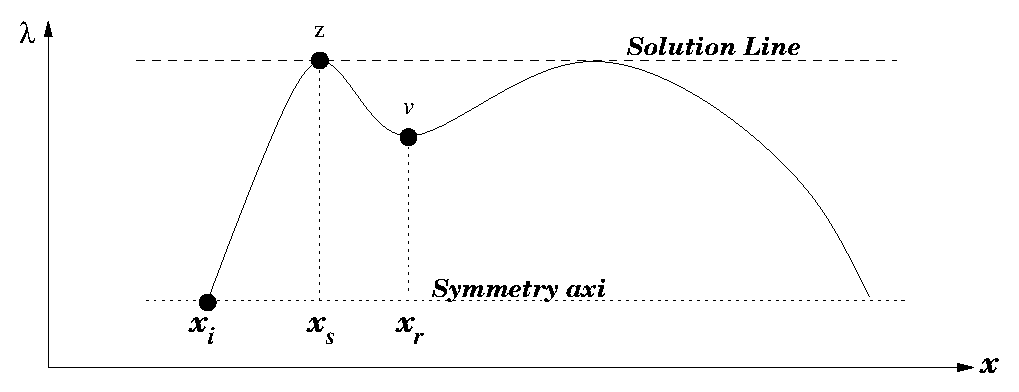
\includegraphics[width=10cm]{nh3figs/radiob.eps}
\caption{Solution point $\rho_s$ and turning point $\rho_r$}
\label{radio1}
\end{figure*}

The slope for the Homotopy path at solution and turning points is zero ($y'={ {d \lambda} \over {dx}} =0$), this property can be used to simplify the expression for the curvature radius at those points, as follows:

\begin{displaymath}
\rho= \Bigg | {1 \over {{ {d^2 \lambda} \over {dx^2}}}} \Bigg |
\end{displaymath}

Now, $\lambda_2$ is derived twice with respect to $x$ from equation \ref{SB2}, considering $a$ and $C$ as constants. After derivation $f(x)$ is superseded by zero because is the solution point, giving as result:

\begin{displaymath}
\rho_{s}=\left[2\,{\frac {\left( x-x_i \right)  \left( x-x_f \right) }{  aC
   \left( {\frac {d}{dx}}f \left( x \right) \right)^{2}}}\right]_{x=x_s}
\end{displaymath}

here $x_s$ is the solution point, $C$ is an arbitrary constant of the Homotopy, and $a$ represents the separation between solution lines.

Equation $\rho_{s}$ allows to conclude that distance $a$ between solution lines affects the acute of the Homotopy path at solutions, in such a way that the curve becomes more sharp as solution lines separates (from each other) and flattens as solution lines unite. Besides, constant $C$ is inversely proportional to the curvature radius.

The point where the path returns to the search of solutions is called turning point $\rho_r$. The study of the curvature radius is completed with the study of the curvature at solutions $\rho_s$ in order to understand in more detail the qualitative behavior of the Homotopy path. At the turning point the derivative of $\lambda$ with respect to $x$ equals zero. Besides, the turning point spatially matches with the critical points of function $f(x)$, so the derivative for $f(x)$ with respect to $x$ is zero. Hence, the equation for the curvature radius is subdivided into the terms shown in Table \ref{ttt}:

\begin{table*}[tbp]
\center{
{\scriptsize
\begin{tabular}{||c||}
\hline\hline
Component    \\ \hline\hline
$r_1=\left[-3/8\, {{ \left( {\frac {C \left( f \left( x \right)  \right) ^{2}}{
 \left( x-x_{{i}} \right) ^{2} \left( x-x_{{f}} \right) }}+{\frac {C
 \left( f \left( x \right)  \right) ^{2}}{ \left( x-x_{{i}} \right) 
 \left( x-x_{{f}} \right) ^{2}}} \right) ^{2}a} \over{ \left( 1-{\frac {C
 \left( f \left( x \right)  \right) ^{2}}{ \left( x-x_{{i}} \right) 
 \left( x-x_{{f}} \right) }} \right) ^{2}}}\right]_{x=x_r}$ \\ \hline
 $r_2=\left[1/4\, {\left( -2\,{\frac {Cf \left( x \right) { { {d^2 f(x)} \over {dx^2}}}}{ \left( x-x_{{
i}} \right)  \left( x-x_{{f}} \right) }}-2\,{\frac {C \left( f \left( 
x \right)  \right) ^{2}}{ \left( x-x_{{i}} \right) ^{3} \left( x-x_{{f
}} \right) }}-2\,{\frac {C \left( f \left( x \right)  \right) ^{2}}{
 \left( x-x_{{i}} \right) ^{2} \left( x-x_{{f}} \right) ^{2}}}-2\,{
\frac {C \left( f \left( x \right)  \right) ^{2}}{ \left( x-x_{{i}}
 \right)  \left( x-x_{{f}} \right) ^{3}}} \right) a \over {\left( 1-{\frac {C
 \left( f \left( x \right)  \right) ^{2}}{ \left( x-x_{{i}} \right) 
 \left( x-x_{{f}} \right) }} \right) }}\right]_{x=x_r}$  \\ \hline
 $r_3=\left[3/8\, {\left( \sqrt {1-{\frac {C \left( f \left( x \right)  \right) ^{2
}}{ \left( x-x_{{i}} \right)  \left( x-x_{{f}} \right) }}}+1 \right) a
 \left( {\frac {C \left( f \left( x \right)  \right) ^{2}}{ \left( x-x
_{{i}} \right) ^{2} \left( x-x_{{f}} \right) }}+{\frac {C \left( f
 \left( x \right)  \right) ^{2}}  { \left( x-x_{{i}} \right)  \left( x-x
_{{f}} \right) ^{2}}} \right) ^{2} \over \left( 1-{\frac {C \left( f \left( 
x \right)  \right) ^{2}}{ \left( x-x_{{i}} \right)  \left( x-x_{{f}}
 \right) }} \right) ^{5/2}}\right]_{x=x_r}$ \\ \hline  
$ r_4=\left[{2\left( \sqrt {1-{\frac {C \left( f \left( x \right)  \right) ^{
2}}{ \left( x-x_{{i}} \right)  \left( x-x_{{f}} \right) }}}+1 \right) 
a \left( {\frac {Cf \left( x \right) { { {d^2 f(x)} \over {dx^2}}}}{ \left( x-x_{{i}}
 \right)  \left( x-x_{{f}} \right) }}+{\frac {C \left( f \left( x
 \right)  \right) ^{2}}{ \left( x-x_{{i}} \right) ^{3} \left( x-x_{{f}
} \right) }}+{\frac {C \left( f \left( x \right)  \right) ^{2}}{
 \left( x-x_{{i}} \right) ^{2} \left( x-x_{{f}} \right) ^{2}}}+{
\frac {C \left( f \left( x \right)  \right) ^{2}}{ \left( x-x_{{i}}
 \right)  \left( x-x_{{f}} \right) ^{3}}} \right) \over 4 \left( 1-{\frac {C
 \left( f \left( x \right)  \right) ^{2}}{ \left( x-x_{{i}} \right) 
 \left( x-x_{{f}} \right) }} \right) ^{3/2}}\right]_{x=x_r}$ \\ \hline   \hline 
\end{tabular}
}
}
\caption{Curvature radius terms of $\rho_{r}$}
\label{ttt}
\end{table*}

The curvature radius is:

\begin{displaymath}
\rho_{r}= {1 \over (r_1+r_2+r_3+r_4)}
\end{displaymath}

Assuming that the second derivative of $f(x)$ with respect to $x$ evaluated at $x_r$ is real and different to zero; the next step is to qualitatively evaluate the behavior of the curvature radius with the following limits:

\begin{equation}
 \displaystyle\lim_{f(x_r) \to{+}\infty}{|\rho_{r}|}=\infty
 \label{rcurv1}
\end{equation}

\begin{equation}
 \displaystyle\lim_{f(x_r) \to{+}0}{|\rho_{r}|}= \infty
  \label{rcurv2}
\end{equation}

\begin{equation}
 \displaystyle\lim_{a \to{+}\infty}{|\rho_{r}|}= 0
  \label{rcurv3}
\end{equation}

\begin{equation}
 \displaystyle\lim_{a \to{+}0}{|\rho_{r}|}= \infty
  \label{rcurv4}
\end{equation}

The limit for equations \ref{rcurv1} and \ref{rcurv2} imply that when $f(x)$ tends to big o very small values, curvature radius grows, so the curve will be flat. As for the case when $f(x)$ has big values (evaluated at turning point $x_r$) is fairly common on the nodal equations of the circuit. Hence, the Homotopy path will tend to remain (flat) close to solution line $\lambda=a$. Since $C$ is being multiplied by $f(x)$, small values for $C$ can be employed in order to reduce the curvature radius. On the other hand, the limits for equations \ref{rcurv3} and \ref{rcurv4} shows that the curvature radius is inversely proportional to the separation value between solution lines $a$. The former suggests that values for $a$ and $C$ can be combined to reduce the proximity of the Homotopy path to the solution line. Finally, all the results for the curvature radius may be extrapolated to the solution line $\lambda=0$ because the symmetry of the paths.

\section{Study cases}

This section will show Homotopy simulations for mathematical and circuital cases in order to expose the new proposed method to a variety of non-linear functions.

\subsection{Mathematical case}

To illustrate the use of Homotopy in a bi-dimensional example, the Homotopy is applied to the following NAEs:

\begin{displaymath}
\begin{array}{c}
f_1(x_1,x_2)=(x_2-1)(x_2-4)(x_2-6)+x_1=0\\
f_2(x_1,x_2)=(x_1-3)(x_1-6)(x_1-9)+x_2=0
\end{array}
\end{displaymath}

where $x_1$ and $x_2$ are variables for the equation system.

Graphical solution of the system is shown in figure \ref{fig:subfig:9sol}.

\begin{figure}[hbtp]
\begin{center}
%% --- first subfigure ---
\subfloat[Five solution system]{
	\label{fig:subfig:9sol}
	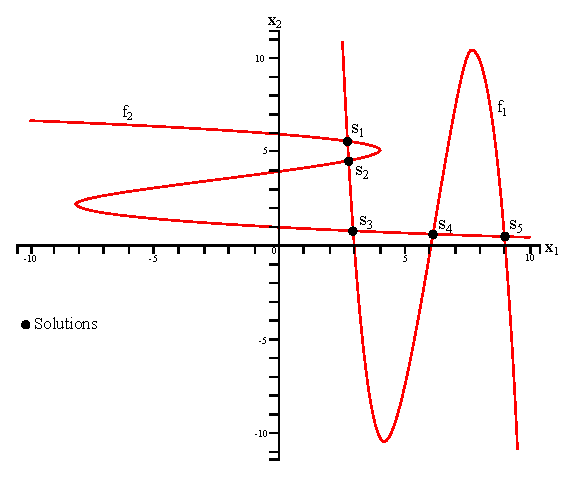
\includegraphics[scale=0.55]{nh3figs/doblelimit_mul_1.eps}}
\hspace{0.3in}
%% --- second subfigure ---
\subfloat[Homotopy path for a two variable example]{
	\label{fig:subfig:homotex}
	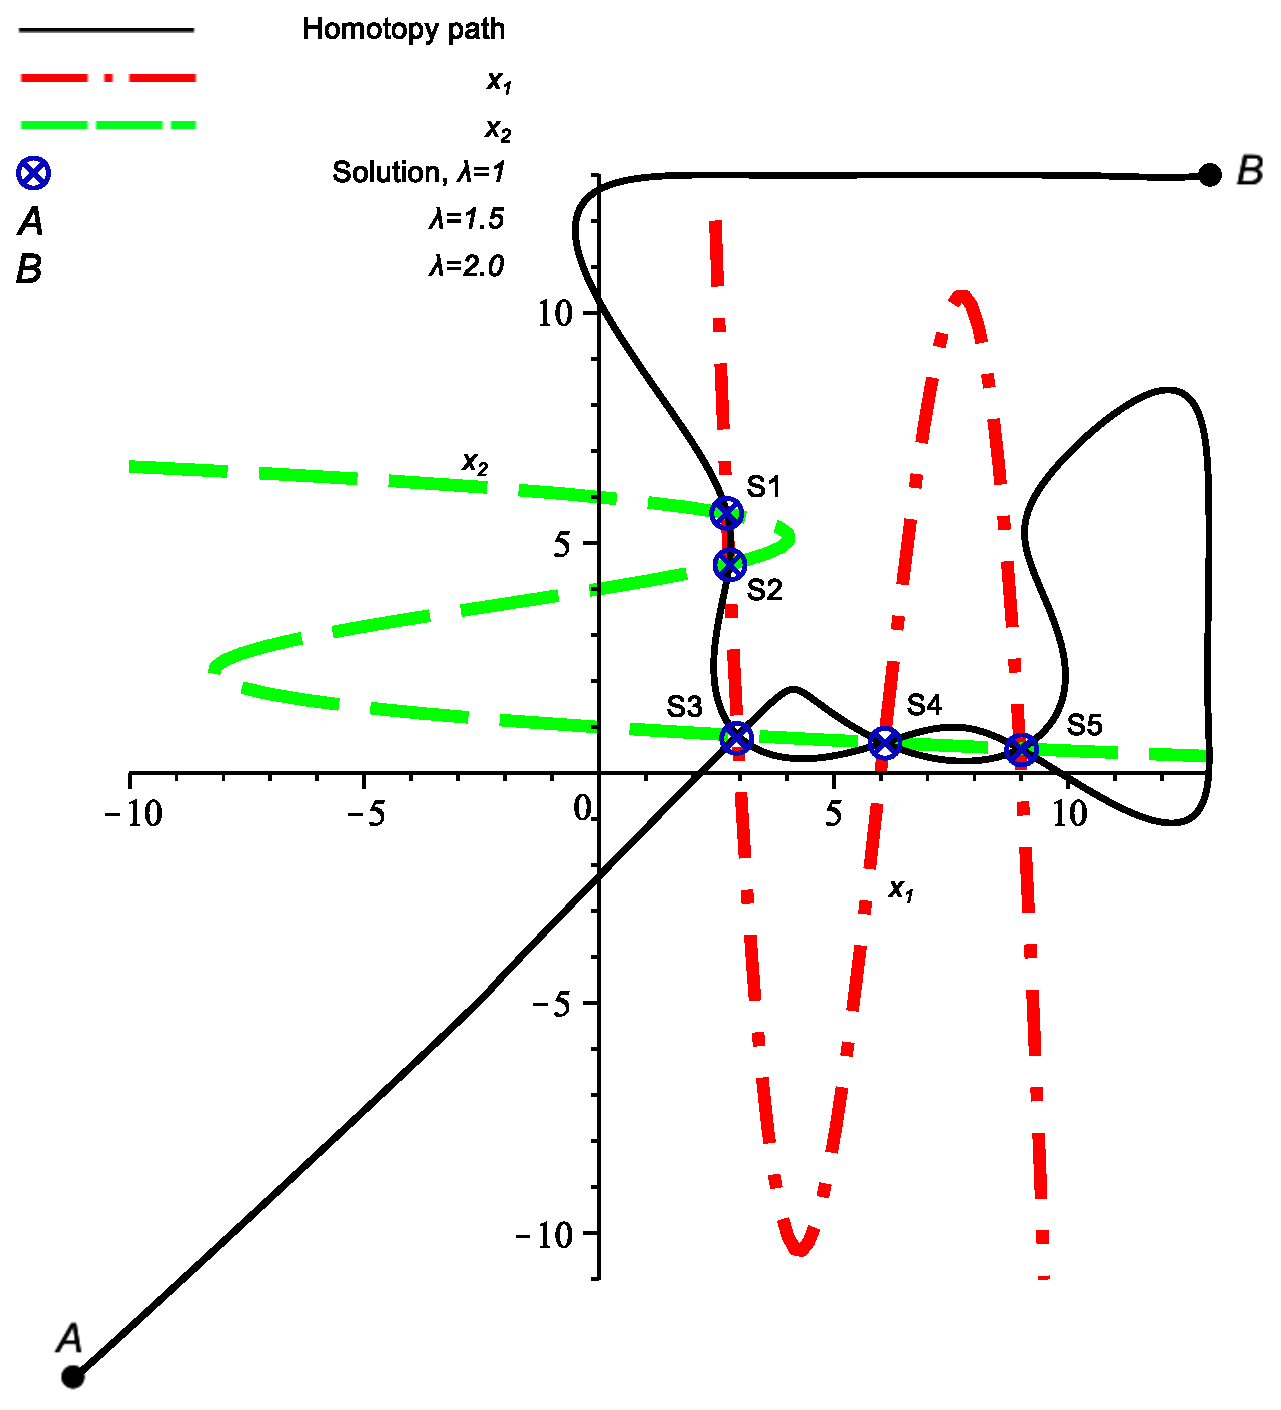
\includegraphics[scale=0.19]{nh3figs/POLINOM2LIMA_1.eps}}
\end{center}
\caption{Mathematical case.}
\label{fig:subfig}
\end{figure}

The proposed Homotopy formulation is:

{\tiny
\begin{displaymath}
\begin{array}{c}
H_1(f_1,\lambda)=\lambda(\lambda-1)(x_1-13)(x_1+13)-(\lambda-0.5)^2 f_1^2=0\\
H_2(f_2,\lambda)=\lambda(\lambda-1)(x_2-13)(x_2+13)-(\lambda-0.5)^2 f_2^2=0\\
\end{array}
\end{displaymath}}

here the solution system is located at $\lambda=0$ and at $\lambda=1$. For practical purposes just one symmetrical branch is employed to trace the Homotopy path, this branch is linked to solution line $\lambda=1$.

As starting point it was chosen $A=(x_1=-13,x_2=-13)$ and path tracing starts, the result is a global convergence for all solutions of the system ($S_1,S_2,S_3,S_4$ y $S_5$) (see figure \ref{fig:subfig:homotex}). The final point is $B=(x_1=13, x_2=13)$ and the Homotopy path for variables $x_1$ and $x_2$ is shown in figures \ref{fig:subfig1:xxx1} and \ref{fig:subfig1:xxx2}, respectively.

\begin{figure*}[hbtp]
\begin{center}
%% --- first subfigure ---
\subfloat[Homotopy path $\lambda-x_1$]{
	\label{fig:subfig1:xxx1}
	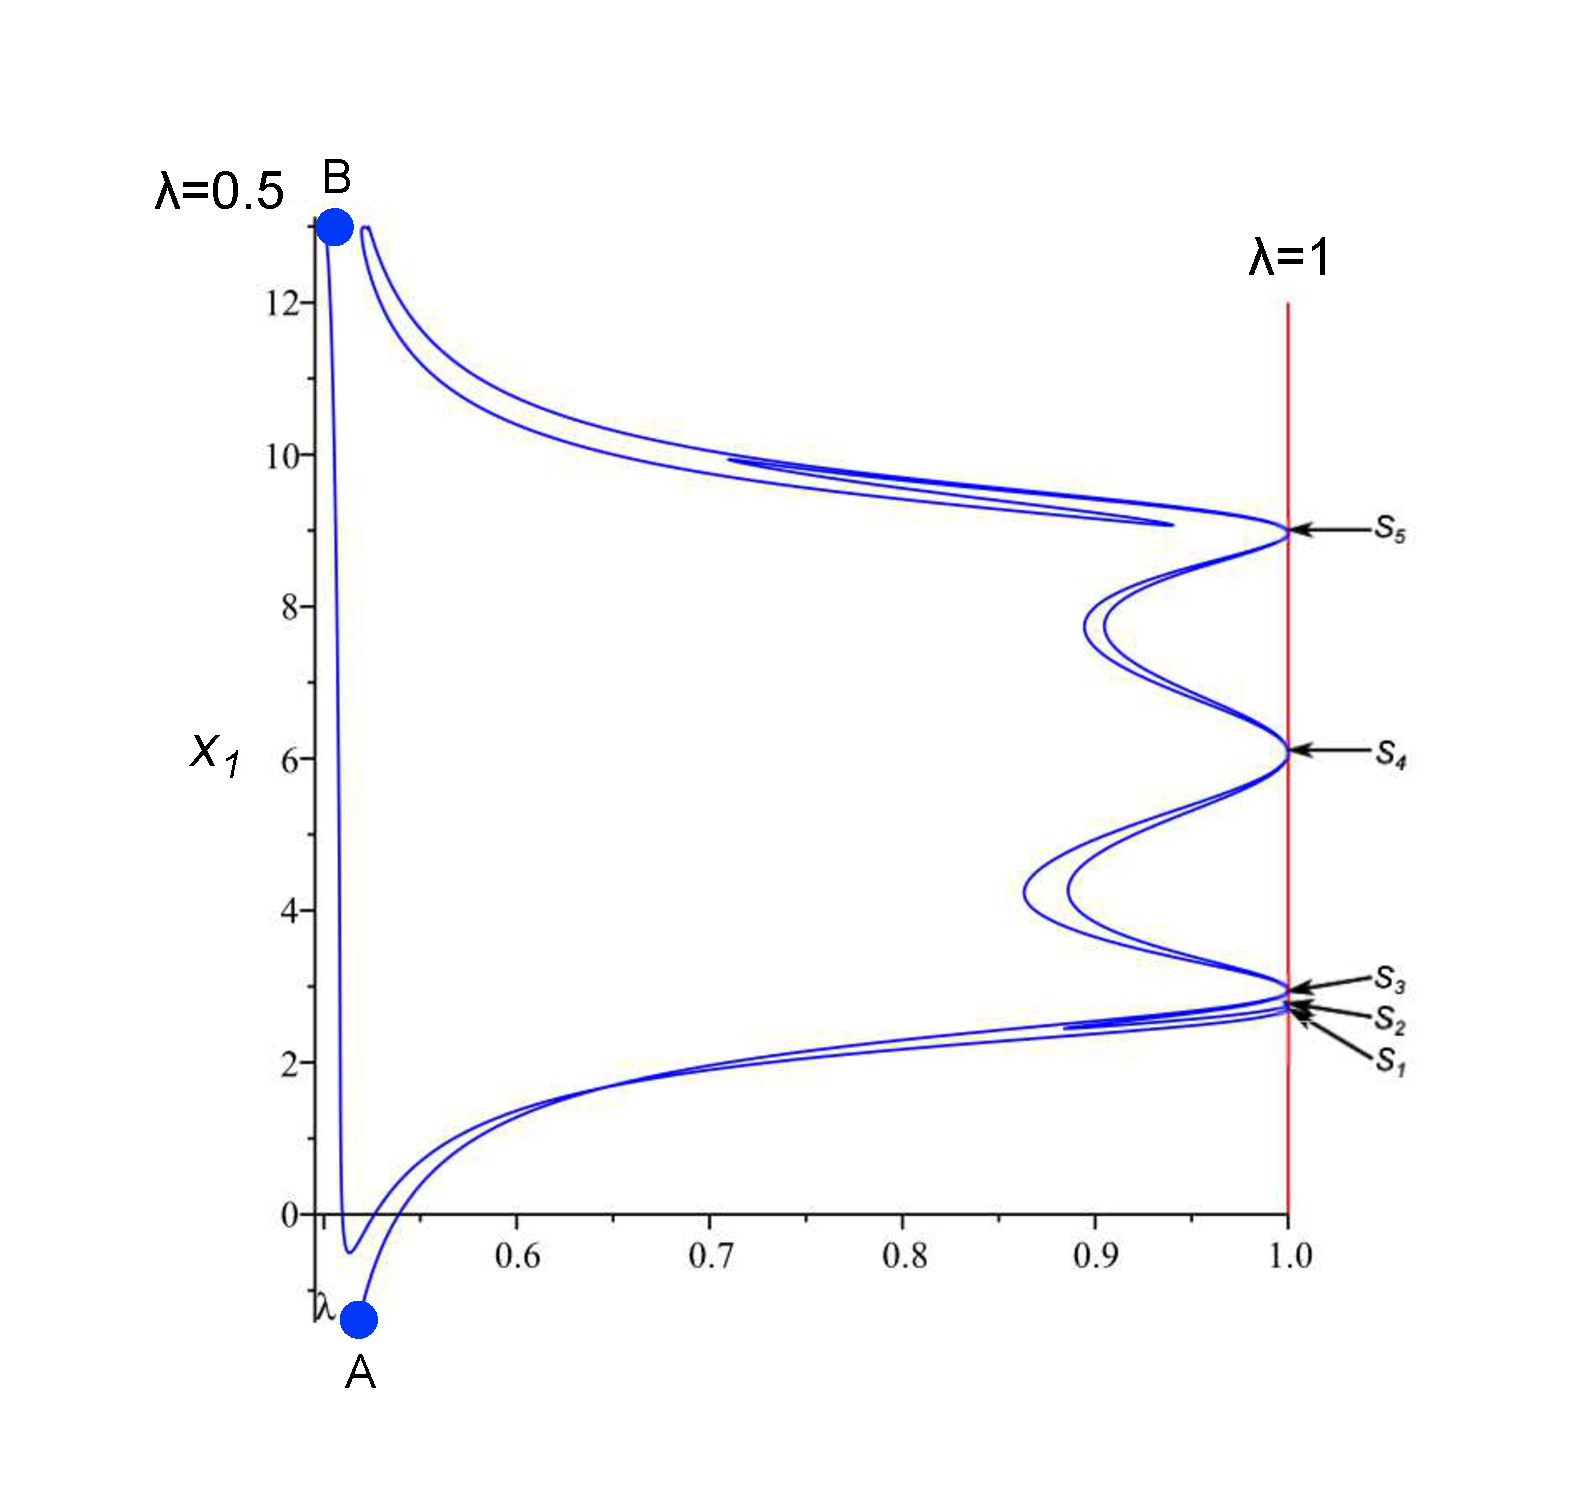
\includegraphics[scale=0.21]{nh3figs/POLINOM2LIMAx1.eps}}
%% --- second subfigure ---
\subfloat[Homotopy path $\lambda-x_2$]{
	\label{fig:subfig1:xxx2}
	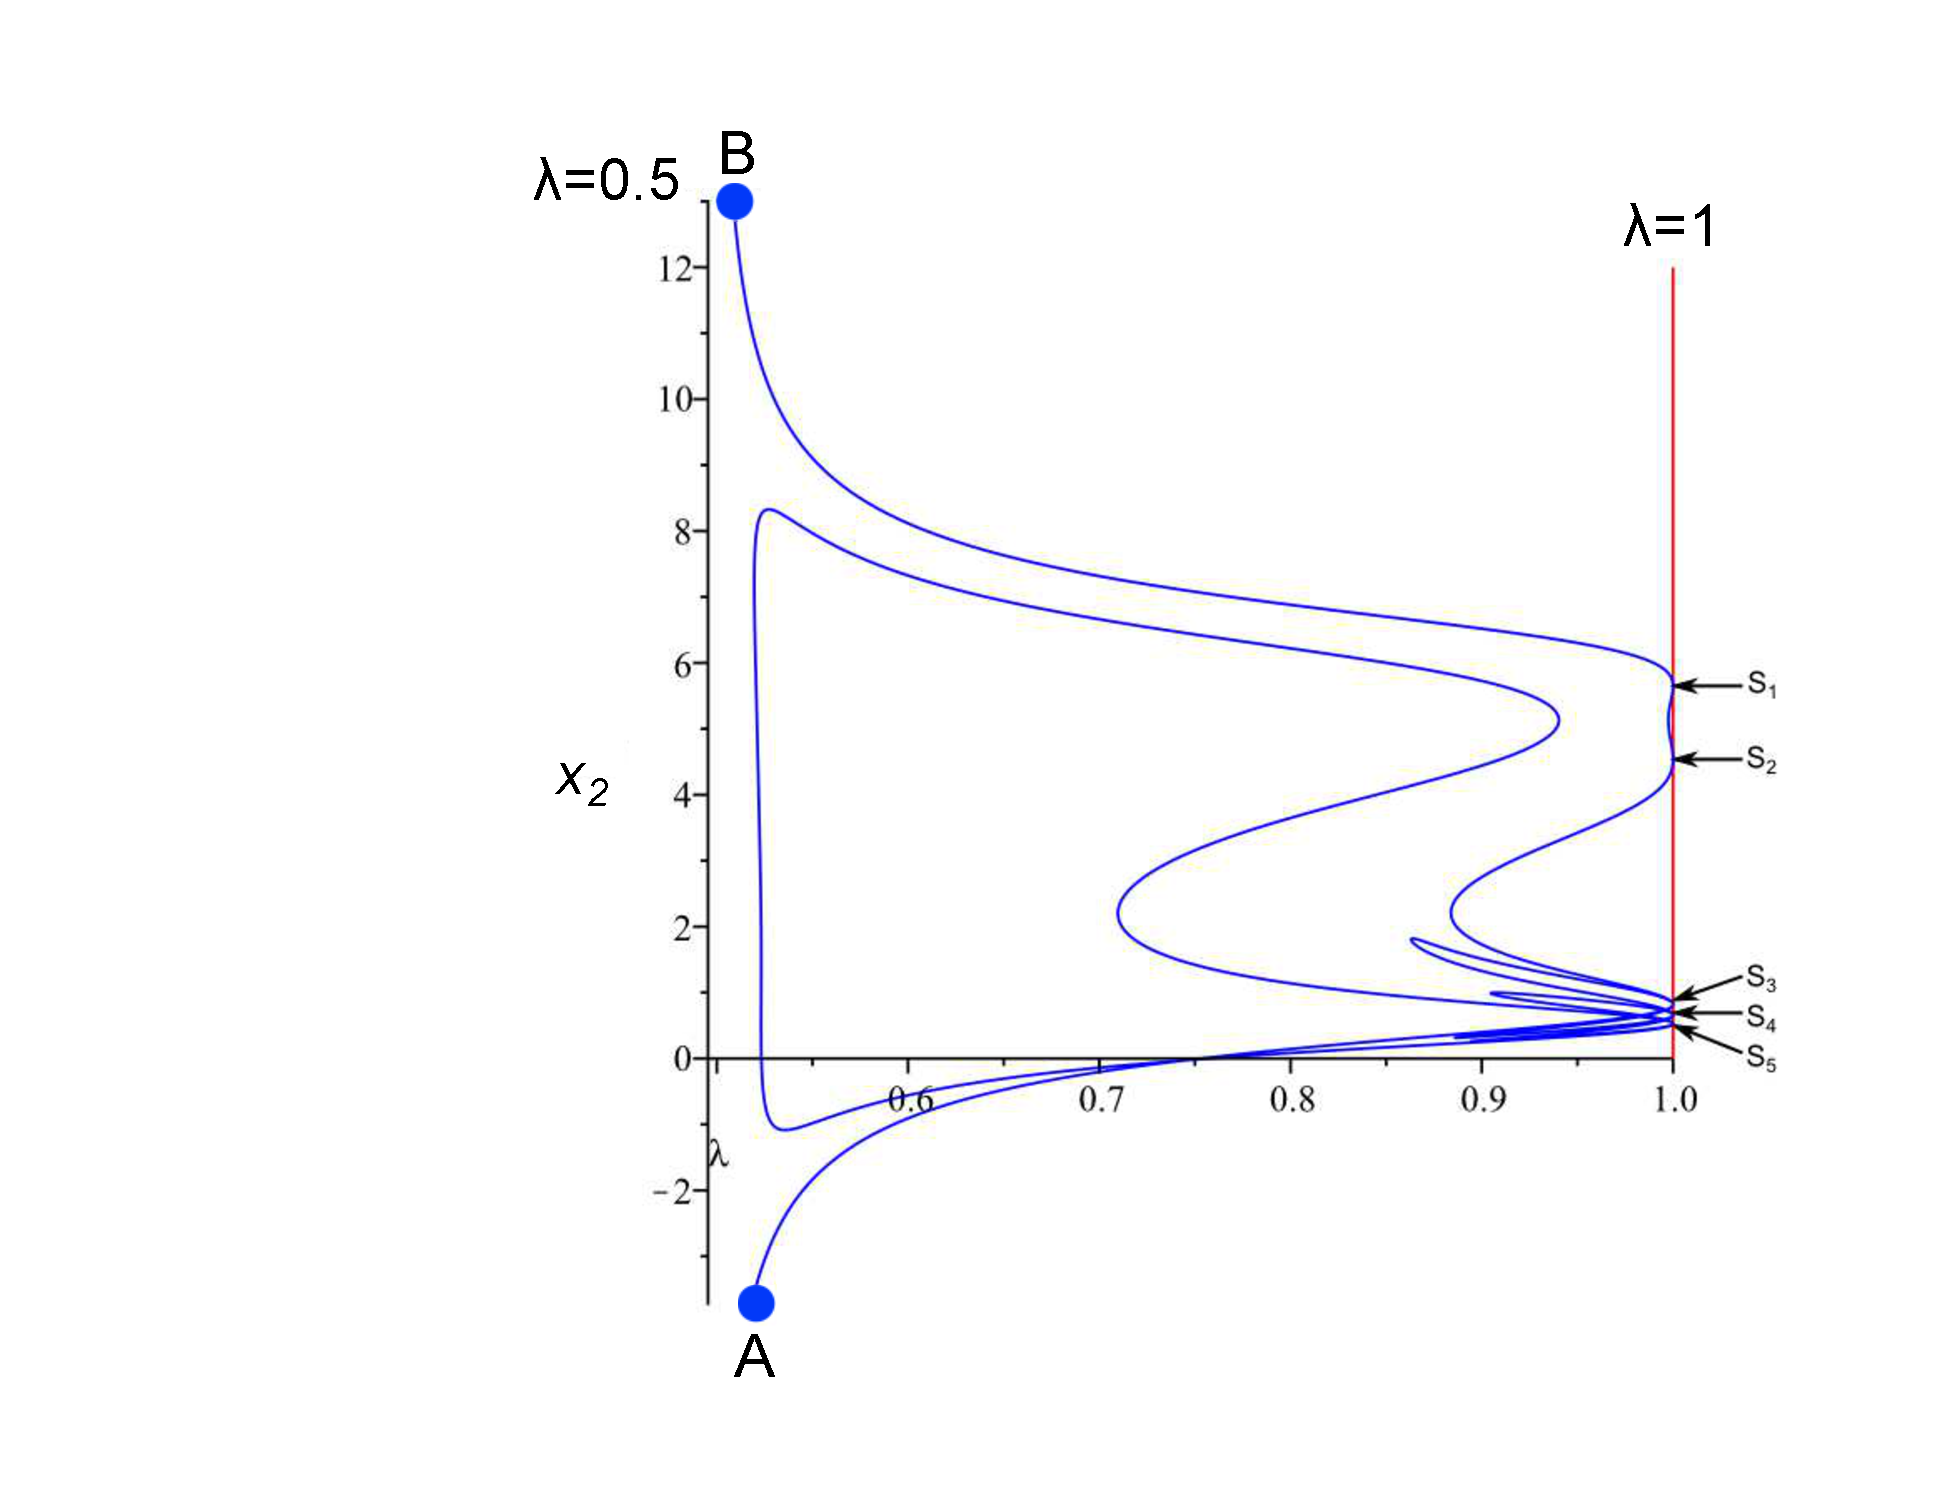
\includegraphics[scale=0.21]{nh3figs/POLINOM2LIMAx2.eps}}
\end{center}
\caption{Homotopic paths.}
\label{fig:subfig1}
\end{figure*}

\subsection{Circuit with two tunnel diodes}

Tunnel diodes have non-linear behavior, which can be described in a general way in figure \ref{fig:subfig2:tunelmod}. As it can be seen in this figure, tunnel diode has 3 sign changes for the slope and combined with a load line could produce up to 3 solutions for a tunnel diode present in the circuit. The model chosen for the tunnel diode in this example is a function of exponential terms \cite{homo_sze},\cite{homo_shur} and can be expressed as:

\begin{displaymath}
i=I_p({V \over V_p})e^{1-{V \over V_p}}+I_0e^{{q \over {KT}} V}
\end{displaymath}

This example presents a circuit (ERDD) with 2 tunnel diodes, one voltage source and one resistor, all of them are in series (see figure \ref{fig:subfig2:2tunel}). The voltage source $V_1$ is at $1V$ and the value for the resistor $R_2$ is $20\Omega$. Besides, both tunnel diodes ($K_3$ and $K_4$) have the same model with coefficients:

$Ip=100 \times 10^{-3}$,
$V_p=50 \times 10^{-3} $, $I_0=1\times 10^{-9}$, and ${q \over {KT}} = 40$. The equilibrium equation is formulated based on the modified nodal analysis (MNA) of the circuit. Also, the system is reduced to 3 equations discarding the nodal voltage $v_1$ because is constant and equals to the voltage source. Therefore, the variables for the resulting system are: $I_E$, $v_2$, and $v_3$. Equations are expressed as follows:

{\tiny
\begin{equation}
\begin{array}{l}
f_1=  {1 \over 20}-{v_2 \over 20}+I_E =0\\ \\
f_2=  -{1 \over 20}+{v_2 \over 20}+2(v_2-v_3)e^{(1-20v_2+20v_3)} \\ +1\times 10^{-9}e^{(40v_2-40v_3)} =0 \\\\
f_3=  2(v_2-v_3)e^{(1-20v_2+20v_3)}+1\times 10^{-9}e^{(40v_2-40v_3)} \\
-2v_3e^{(1-20v_3)}-1\times 10^{-9} e^{(40v_3)} =0 
\end{array} 
\end{equation}}

\begin{figure}[hbtp]
\begin{center}
%% --- first subfigure ---
\subfloat[Tunnel diode model]{
	\label{fig:subfig2:tunelmod}
	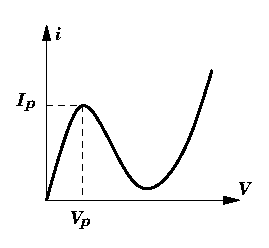
\includegraphics[scale=1]{nh3figs/tunnelmod.eps}}
\hspace{0.3in}
%% --- second subfigure ---
\subfloat[Circuit with two tunnel diodes]{
	\label{fig:subfig2:2tunel}
	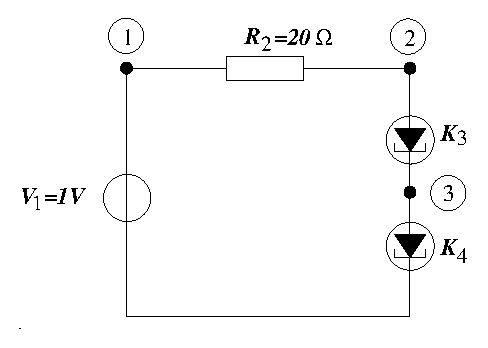
\includegraphics[scale=0.5]{nh3figs/erdd.eps}}
\end{center}
\caption{Example with tunnel diodes.}
\label{fig:subfig2}
\end{figure}

Now, the DBH is applied to solve the circuit. The Homotopy formulation is given as:

{\tiny
\begin{displaymath}
\begin{array}{c}
H_1(f_1,\lambda)=\lambda(\lambda-1)(I_E-1)(I_E+1)-(\lambda-0.5)^2 f_1^2=0\\
H_2(f_2,\lambda)=\lambda(\lambda-1)(v_2-1)(v_2+1)-(\lambda-0.5)^2 f_2^2=0\\
H_3(f_3,\lambda)=\lambda(\lambda-1)(v_3-1)(v_3+1)-(\lambda-0.5)^2 f_3^2=0\\
\end{array}
\end{displaymath}
}
where the bounding lines are $a=0$ and $b=1$, and the initial point for the Homotopy path is selected as $A=[I_E=-1,v_2=-1,v_3=-1,\lambda=0.5]$.


As result of the tracing for the Homotopy path, all the operating points of the circuit are located, nine
in total (Figure \ref{2tunelg}(a)). In order to make the results clearer, Homotopy path and the equilibrium equation are presented
as function of the branch voltages ($u_2=v_2-v_3$ y $u_3=v_3$) of the tunnel diodes. This depiction
allows to trace the homotopy path in terms of the branch functions of the tunnel diodes.
Figure \ref{2tunelg}(a) shows the complete symmetric
path associated to the bounding line $\lambda = 1$ against branch current $u_2$.
Besides, the final point for the path was located at $B=[I_E=1,v_2=1,v_3=1, \lambda=0.5]$. Figure \ref{2tunelg}(b) shows a close-up to the solutions region, here can be seen how the path crosses through all 9 solutions, this presents 3 regions ($F1$, $F2$ y $F3$) of close roots. To observe in detail the behavior of the path, a close-up for every one of regions $F1$, $F2$, and $F3$ is performed, these are shown in figures \ref{2tunelg}(c), \ref{2tunelg}(d), and \ref{2tunelg}(e)), respectively. In those figures all solutions are shown found by the Homotopy path.
 
\begin{figure*}[hbtp]
\centering
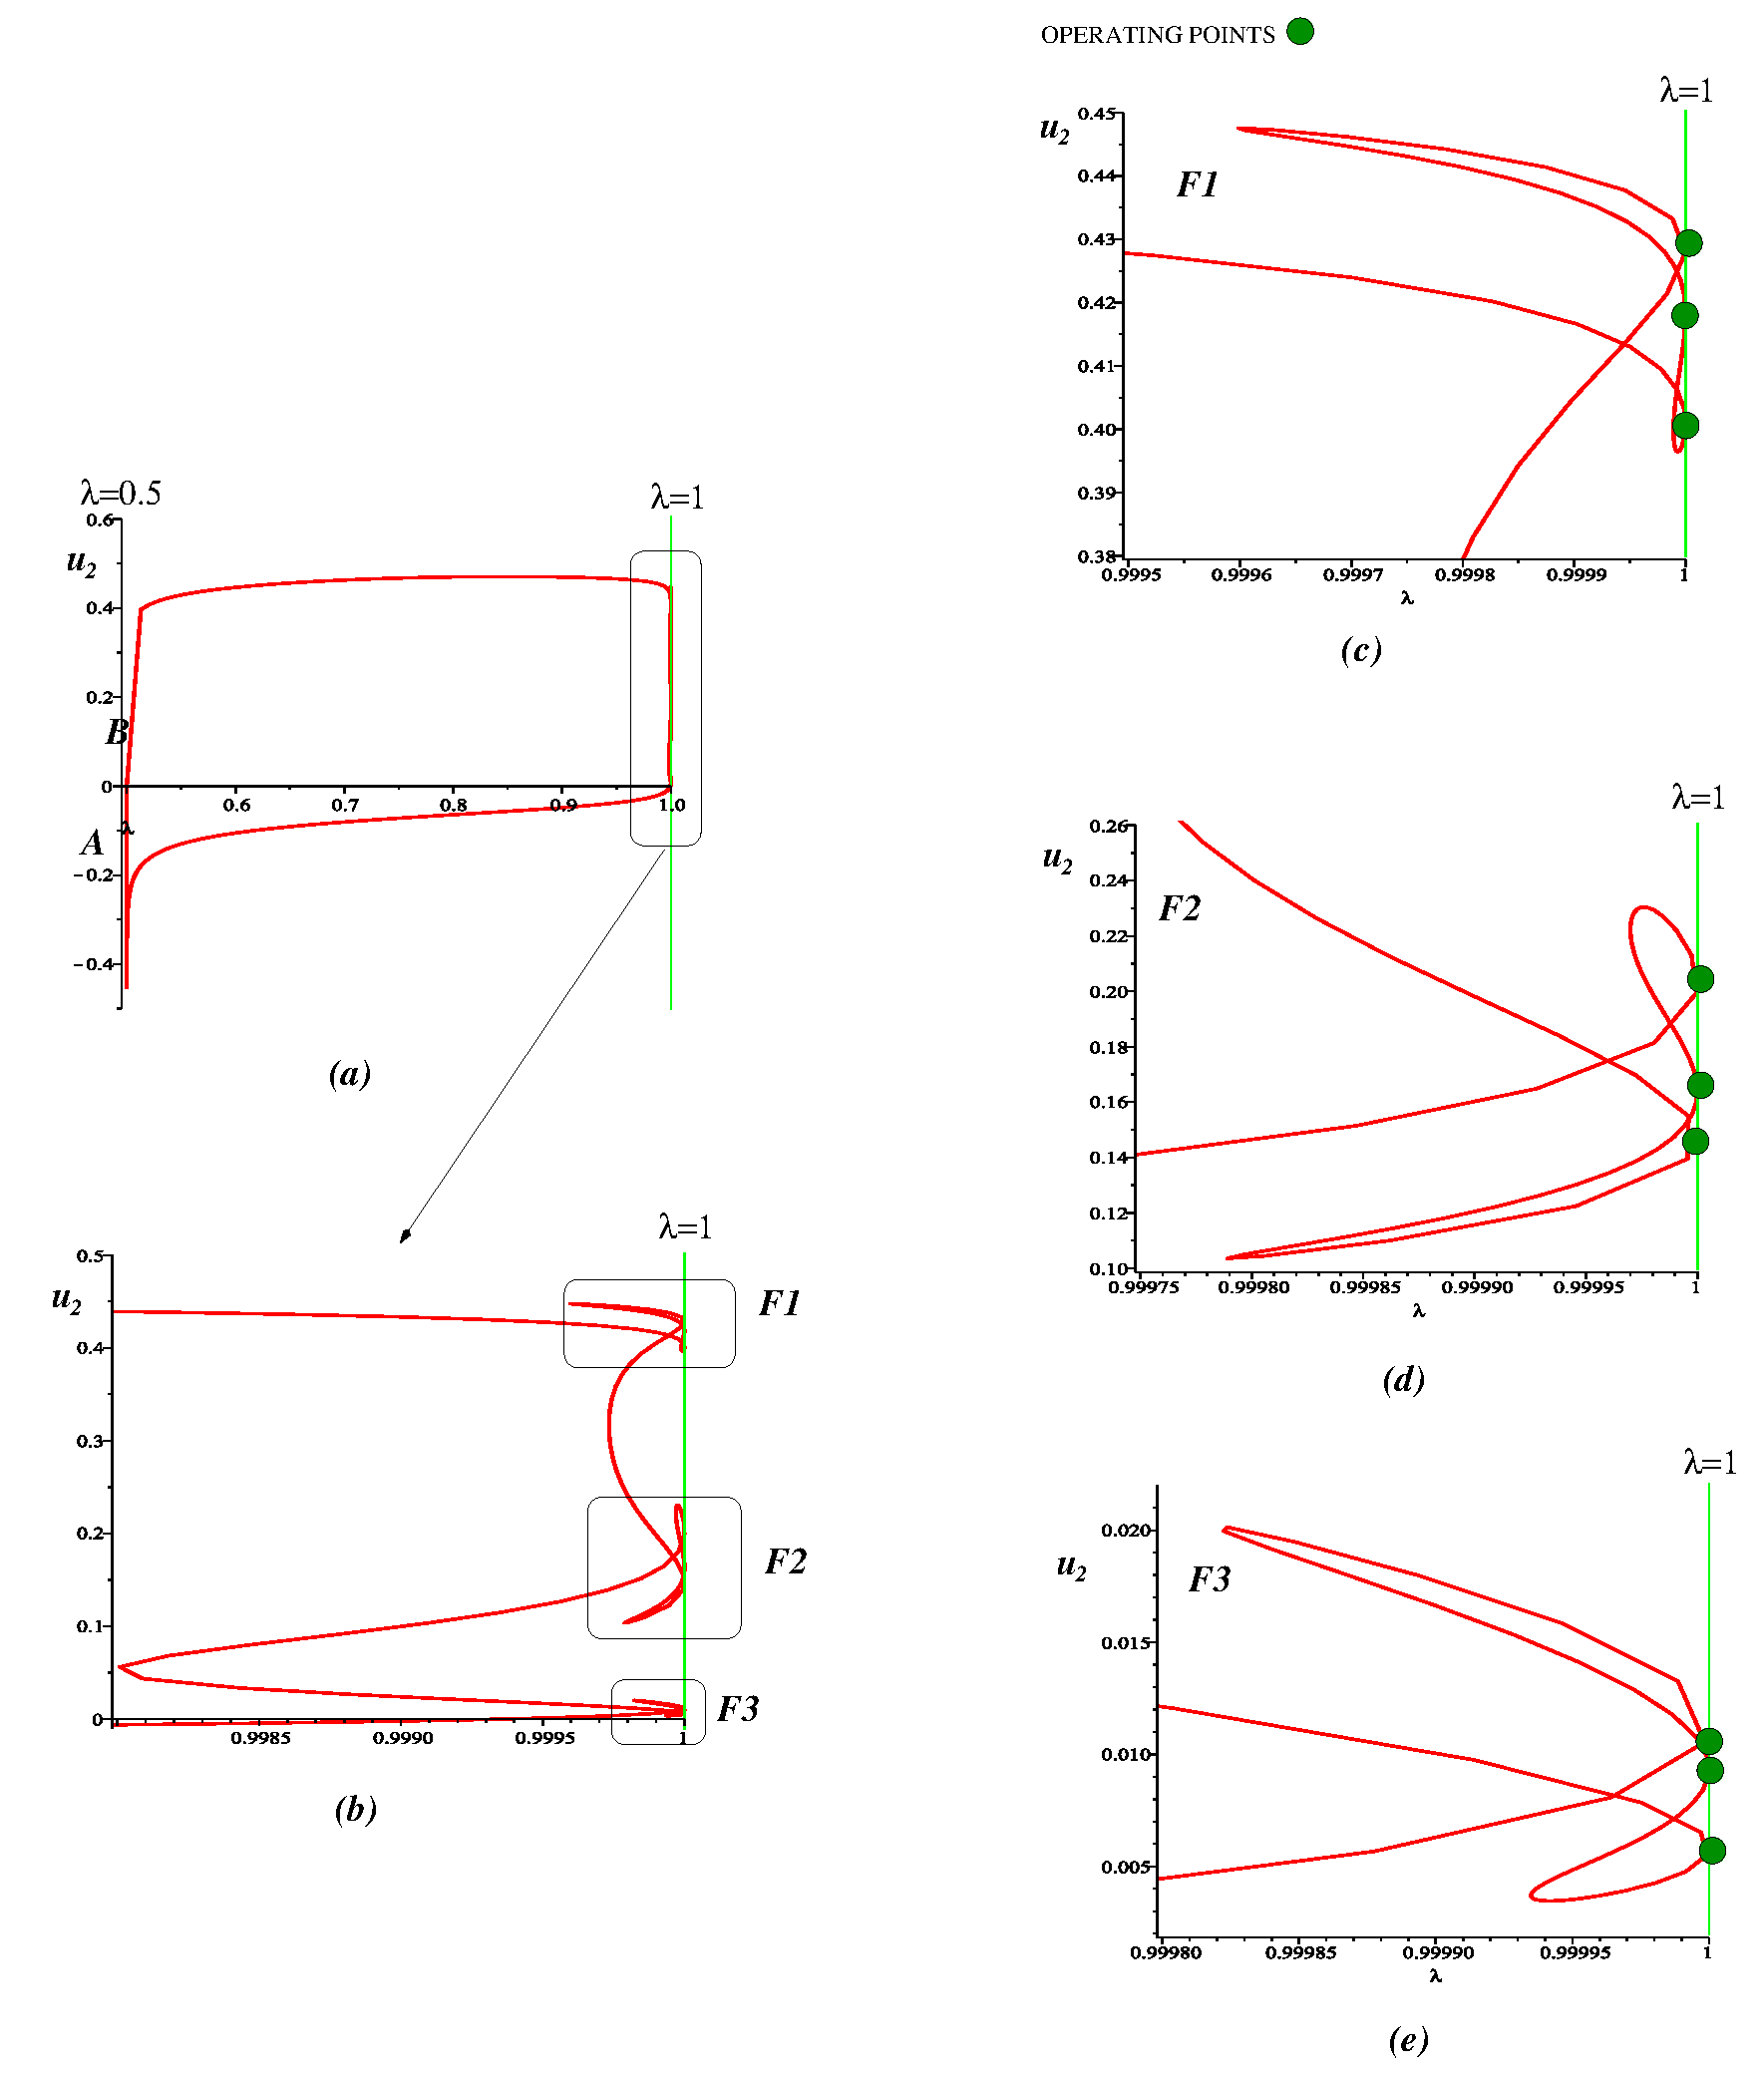
\includegraphics[scale=0.3]{nh3figs/diodos/diodo.eps}
\caption{Homotopy path ($u_2$-$\lambda$) for the circuit with tunnel diodes.}
\label{2tunelg}
\end{figure*}

\subsection{Circuit with bipolar transistors and a diode}

A circuit with bipolar transistors and a diode was reported by \cite{homo_tadeusiewicz} and  \cite{homo_yamamurawise}, it was originally solved using piecewise methods. Then, in \cite{homo_yamamura}, the circuit was solved by fixed point modified Homotopy. This circuit has 3 operating points. All transistors are modeled using Ebers-Moll. The equation of this model is:

\begin{displaymath}
\left[ \begin{array}{c}
i_{D_E} \\
i_{D_C}
\end{array}\right] =
\left[ \begin{array}{cc} 1  & \alpha_R \\
\alpha_F & 1 \\
\end{array}\right] \left[ \begin{array}{c}
10^{-9}(e^{(40v_{be})} - 1) \\
10^{-9}(e^{(40v_{bc})} - 1)
\end{array}\right]
\end{displaymath}

The circuital depiction of the model is shown in figure \ref{FEbersMoll}.

The model for the diode is:

\begin{displaymath}
i_d=10^{-9}(e^{40u} - 1)
\end{displaymath}

\begin{figure*}[tbp]
\centerline{
\epsfxsize=90mm
\epsffile{nh3figs/diotran.eps}
}
\caption{Circuit with bipolar transistors and a diode.}
\label{yamamuracircuito}
\end{figure*}

\begin{figure}[hbtp]
\psfrag{f}{$\alpha_F$}
\psfrag{r}{$\alpha_R$}
\centerline{
\epsfxsize=2mm
\epsffile{nh3figs/ebersmoll.eps}}
\caption{Ebers-Moll model for the bipolar transistor.}
\label{FEbersMoll}
\end{figure}

The values for the components in the circuit can be found in table \ref{yamamuracircuitovalores}. First, equilibrium equation is formulated using the modified nodal analysis resulting in a system with 14 equations and 14 variables. The circuit is shown in figure \ref{yamamuracircuito} and its nodal equations  (Equilibrium Equations) are shown on table \ref{eqsd} (using MNA analysis).

\begin{table}[hbtp]
\center{
{\scriptsize
\begin{tabular}{||c|c||}
\hline\hline
Component  & Value  \\ \hline\hline
$R_1$ & $4K\Omega$   \\ \hline
$R_2$ & $0.1K\Omega$   \\ \hline
$R_3$ & $8K\Omega$   \\ \hline
$R_4$ & $8K\Omega$   \\ \hline
$R_5$ & $4K\Omega$   \\ \hline
$R_6$ & $0.1K\Omega$   \\ \hline
$R_7$ & $30K\Omega$   \\ \hline
$R_8$ & $1K\Omega$   \\ \hline
$R_9$ & $0.1K\Omega$   \\ \hline
$R_{10}$ & $10K\Omega$   \\ \hline
$R_{11}$ & $4K\Omega$   \\ \hline
$R_{12}$ & $10K\Omega$   \\ \hline
$R_{13}$ & $1K\Omega$   \\ \hline
$V_{cc}$ & $12V$   \\ \hline  \hline
\end{tabular}
}
}
\caption{Circuit components.}
\label{yamamuracircuitovalores}
\end{table}



\begin{table*}[tbp]
{\tiny
\begin{tabular}{|r||r|}  \hline\hline
$f_1$ & ${\frac {37}{20000}}\,{\it v_1}-{\frac {1}{4000}}\,{\it v_2}-{\frac {1}{
 4000}}\,{\it v_6}-{\frac {1}{1000}}\,{\it v_9}-{\frac {1}{4000}}\,{\it 
v_{12}}-{\frac {1}{10000}}\,{\it v_{13}}+{\it IE}=0$ \\  
$f_2$ & $-{\frac {1}{4000}}\,{\it v_1}+{\frac {3}{8000}}\,{\it v_2}-{\frac {1}{
8000}}\,{\it v_5}+ 0.00000000990\,{{\rm e}^{40\,{\it v_4}-40\,{\it v_3}}}
+ 0.00000000010- 0.000000010\,{{\rm e}^{40\,{\it v_4}-40\,{\it v_2}}}=0$  \\  
$f_3$ & ${\frac {1}{100}}\,{\it v_3}- 0.000000010\,{{\rm e}^{40\,{\it v_4}-40\,{
\it v_3}}}+ 0.00000000990+ 0.00000000010\,{{\rm e}^{40\,{\it v_4}-40\,{
\it v_2}}}=0$ \\
$f_4$ & ${\frac {1}{8000}}\,{\it v_4}-{\frac {1}{8000}}\,{\it v_6}+ 0.00000000010
\,{{\rm e}^{40\,{\it v_4}-40\,{\it v_3}}}- 0.00000001000+ 0.00000000990
\,{{\rm e}^{40\,{\it v_4}-40\,{\it v_2}}}=0$ \\
$f_5$ & $-{\frac {1}{8000}}\,{\it v_2}+{\frac {1}{8000}}\,{\it v_5}+
 0.00000000010\,{{\rm e}^{40\,{\it v_5}-40\,{\it v_7}}}- 0.00000001000+
 0.00000000990\,{{\rm e}^{40\,{\it v_5}-40\,{\it v_6}}}=0$ \\
$f_6$ & $-{\frac {1}{4000}}\,{\it v_1}-{\frac {1}{8000}}\,{\it v_4}+{\frac {3}{
8000}}\,{\it v_6}+ 0.00000000990\,{{\rm e}^{40\,{\it v_5}-40\,{\it v_7}}}
+ 0.00000001010- 0.000000010\,{{\rm e}^{40\,{\it v_5}-40\,{\it v_6}}}-
 0.000000010\,{{\rm e}^{40\,{\it v_8}-40\,{\it v_6}}}=0$ \\
$f_7$ & ${\frac {1}{100}}\,{\it v_7}- 0.000000010\,{{\rm e}^{40\,{\it v_5}-40\,{
\it v_7}}}+ 0.00000000990+ 0.00000000010\,{{\rm e}^{40\,{\it v_5}-40\,{
\it v_6}}}=0$ \\
$f_8$ & ${\frac {1}{30000}}\,{\it v_8}-{\frac {1}{30000}}\,{\it v_9}+ 0.000000010
\,{{\rm e}^{40\,{\it v_8}-40\,{\it v_6}}}- 0.000000010=0$ \\
$f_9$ & $-{\frac {1}{1000}}\,{\it v_1}-{\frac {1}{30000}}\,{\it v_8}+{\frac {31}{
30000}}\,{\it v_9}+ 0.00000000990\,{{\rm e}^{40\,{\it v_{11}}-40\,{\it v_{10}
}}}+ 0.00000000010- 0.000000010\,{{\rm e}^{40\,{\it v_{11}}-40\,{\it v_9}}
}=0$ \\
$f_{10}$ & ${\frac {1}{100}}\,{\it v_{10}}- 0.000000010\,{{\rm e}^{40\,{\it v_{11}}-40\,
{\it v_{10}}}}+ 0.00000000990+ 0.00000000010\,{{\rm e}^{40\,{\it v_{11}}-40
\,{\it v_9}}}=0$ \\
$f_{11}$ & ${\frac {1}{10000}}\,{\it v_{11}}-{\frac {1}{10000}}\,{\it v_{12}}+
 0.00000000010\,{{\rm e}^{40\,{\it v_{11}}-40\,{\it v_{10}}}}- 0.00000001000
+ 0.00000000990\,{{\rm e}^{40\,{\it v_{11}}-40\,{\it v_9}}}=0$ \\
$f_{12}$ & $-{\frac {1}{4000}}\,{\it v_1}-{\frac {1}{10000}}\,{\it v_{11}}+{\frac {7}{
20000}}\,{\it v_{12}}+ 0.00000000990\,{{\rm e}^{40\,{\it v_{13}}}}+
 0.00000000010- 0.000000010\,{{\rm e}^{40\,{\it v_{13}}-40\,{\it v_{12}}}}=0$ \\
$f_{13}$ & $-{\frac {1}{10000}}\,{\it v_1}+{\frac {11}{10000}}\,{\it v_{13}}+
 0.00000000010\,{{\rm e}^{40\,{\it v_{13}}}}- 0.00000001000+
 0.00000000990\,{{\rm e}^{40\,{\it v_{13}}-40\,{\it v_{12}}}}=0$ \\
$f_{14}$ & $v_1-12=0$ \\ \hline\hline
\end{tabular}}
\caption{Nodal equations}
\label{eqsd}
\end{table*}


Now, the DBH is applied to solve the circuit. The Homotopy formulation is expressed as follows:

{\tiny
\begin{displaymath}
\begin{array}{c}
H_1(f_1,\lambda)=\lambda(\lambda-1)(v_1-13)(v_1+13)-C(\lambda-0.5)^2 f_1^2=0\\
H_2(f_2,\lambda)=\lambda(\lambda-1)(v_2-13)(v_2+13)-C(\lambda-0.5)^2 f_2^2=0\\
\vdots \\
H_{14}(f_{14},\lambda)=\lambda(\lambda-1)(I_E-13)(I_E+13)-C(\lambda-0.5)^2 f_{14}^2=0\\
\end{array}
\end{displaymath}
}
where the constant value $C$ is $C=0.1$, bounding lines are $a=0$ and $b=1$, and the initial point of the Homotopy path is selected as shown in table \ref{iniyama}. Then, the circuit is solved using double bounded Homotopy, resulting in the convergence to the 3 known solutions for the circuit. The Homotopy path that corresponds to the current for the voltage source $I_E$ is shown in figure \ref{yamaie}. Finally, the final point for the Homotopy trace is shown in table \ref{iniyama}.

\begin{table*}[tbp]
{\small
\center{
\hspace{-4mm}
\begin{tabular}{||c|c|c|c|c|c|c|c|c|c|c|c|c|c|c||}
\hline\hline
Point & $v_1$ & $v_2$ & $v_3$ & $v_4$ & $v_5$ & $v_6$ & $v_7$ & $v_8$ & $v_9$ & $v_{10}$& $v_{11}$ & $v_{12}$ & $v_{13}$ & $i_E$ \\ \hline
Initial $\pig{x_i}$ &  +13 & -13 & -13 & -13 & -13 & -13 & -13 & -13 & -13 & -13 & -13 & -13 & -13 & -13  \\ \hline
Final $\pig{x_f}$ &  +13 & +13 & -13 & -13 & +13 & +13 & +13 & +13 & -13 & +13 & -13 & -13 & -13 & +13  \\ \hline
\end{tabular}
}
}
\caption{Initial and final point for the Homotopy path for the circuit in figure \ref{yamamuracircuito}.}
\label{iniyama}
\end{table*}

\begin{table*}[tbp]
{\small
\center{
\hspace{-4mm}
\begin{tabular}{||c|c|c|c|c|c|c|c|c|c|c|c|c|c|c||}
\hline\hline
Sol & $v_1$ & $v_2$ & $v_3$ & $v_4$ & $v_5$ & $v_6$ & $v_7$ & $v_8$ & $v_9$ & $v_{10}$& $v_{11}$ & $v_{12}$ & $v_{13}$ & $i_E$ \\ \hline
$S_1$ &  12 & 5.995 & 0.085 &0.368 &0.712 &0.436 &0.390 &0.699 &11.635 &0.4e-5 &0.039 &0.039 &0.321 &-0.0089 \\ \hline
$S_2$ & 12 & 0.883 & 0.278 &0.590 &0.631 &0.812 &0.315 &1.074 &11.647 &0.4e-5 &0.039 &0.039 &0.321 &-0.0100 \\ \hline
$S_3$ & 12 & 0.405 & 0.366 &0.685 &0.349 &6.796 &0.070 &7.038 &11.839 &0.4e-5 &0.039 &0.039 &0.321 &-0.0085 \\ \hline \hline
\end{tabular}
}
}
\caption{Operating points (solutions) for figure \ref{yamamuracircuito}.}
\label{yamamuracircuitosoluc}
\end{table*}


\begin{figure}[hbtp]
\begin{center}
	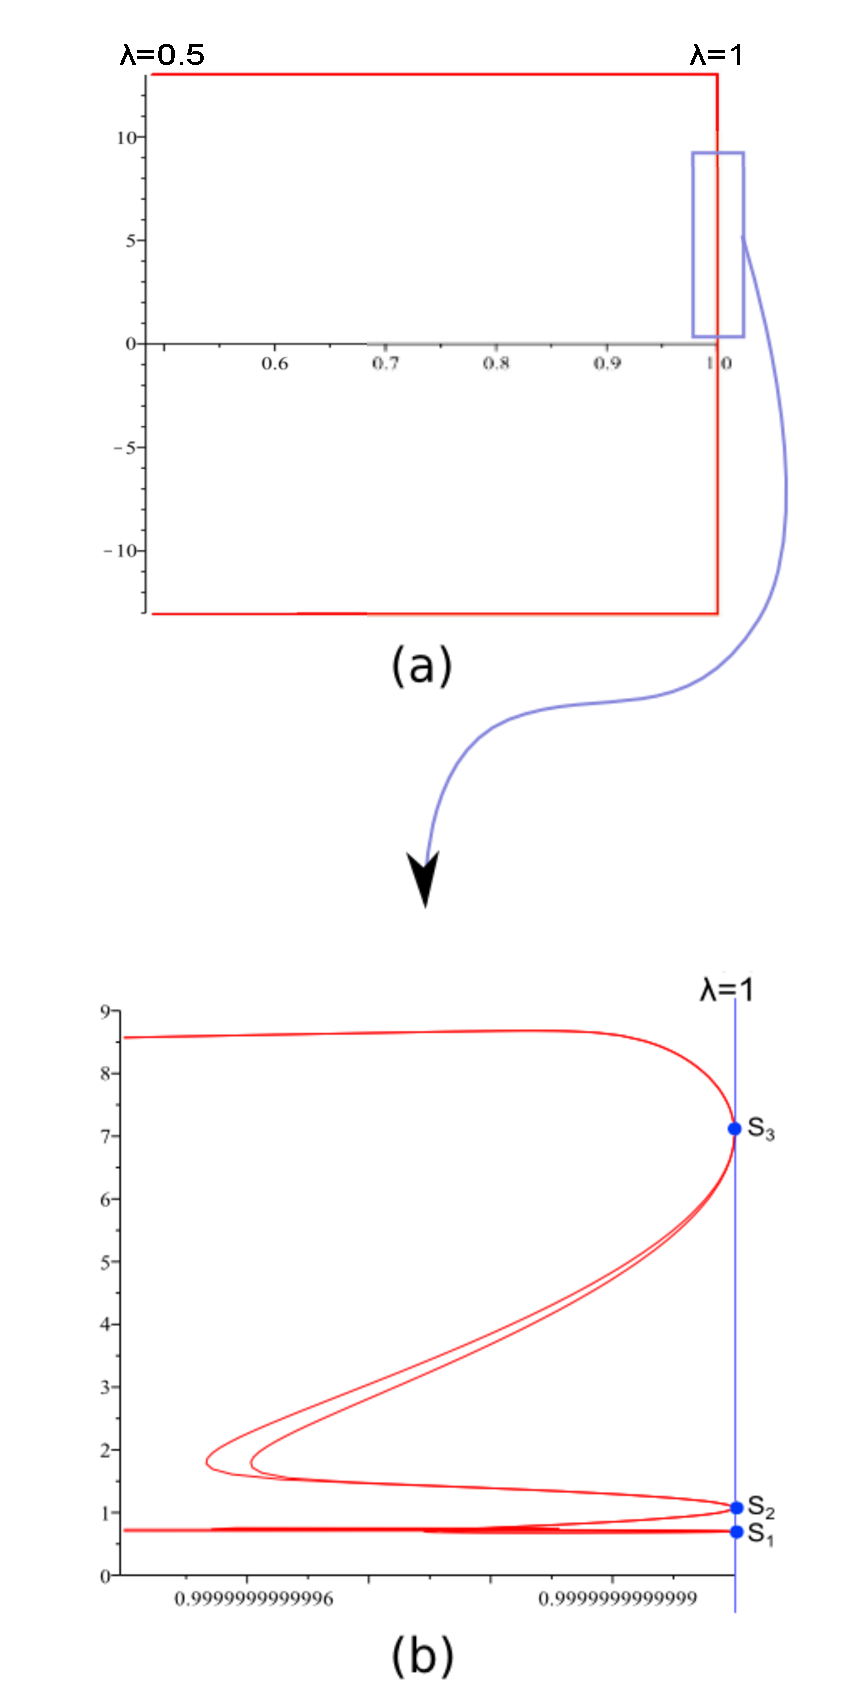
\includegraphics[scale=.4]{nh3figs/YAMAMURAV8_FULL.eps}
\end{center}
\caption{Homotopy path $\lambda-v_8$}
\label{yamaie}
\end{figure}

\subsection{Chua's circuit}

The following circuit \cite{homo_chua} (see figure \ref{fig:subfig3:chua}), contains 9 solutions, has become the reference circuit for the Homotopy applied to circuit analysis. Values of the components are shown in figure \ref{chuatablet}. This circuit has 4 bipolar transistors modeled using Ebers-Moll for the bipolar transistor operating in the direct active region (see figure \ref{fig:subfig3:eber}).

\begin{table}[hbtp]
\center{
{\scriptsize
\begin{tabular}{||c|c|c|c||}
\hline\hline
Component  & Value  & Component & Value\\ \hline\hline
$R_1$ & $1k\Omega$ & $R_9$ & $10.1k\Omega$    \\ \hline
$R_2$ & $4k\Omega$ & $R_{10}$ & $10.1k\Omega$  \\ \hline
$R_3$ & $4k\Omega$  &  $R_{11}$ & $4k\Omega$  \\ \hline
$R_4$ & $5k\Omega$  &  $R_{12}$ & $4k\Omega$  \\ \hline
$R_5$ &  $30k\Omega$ & $R_{13}$ & $30k\Omega$    \\ \hline
$R_6$  & $0.5k\Omega$ & $R_{14}$ & $30k\Omega$  \\ \hline
$R_7$ & $0.5k\Omega$  &  $V_1$ & $10V$  \\ \hline
$R_8$ & $30k\Omega$  &  $V_2$ & $2V$  \\ \hline
$V_{CC}$ & $12V$  &  $\alpha$& $0.98$     \\ \hline\hline
\end{tabular}
}
}
\caption{Values of the components for the circuit shown in figure \ref{fig:subfig3:chua}.}
\label{chuatablet}
\end{table}

\begin{figure*}[hbtp]
\begin{center}
%% --- first subfigure ---
\subfloat[Chua's circuit with 9 solutions.]{
	\label{fig:subfig3:chua}
	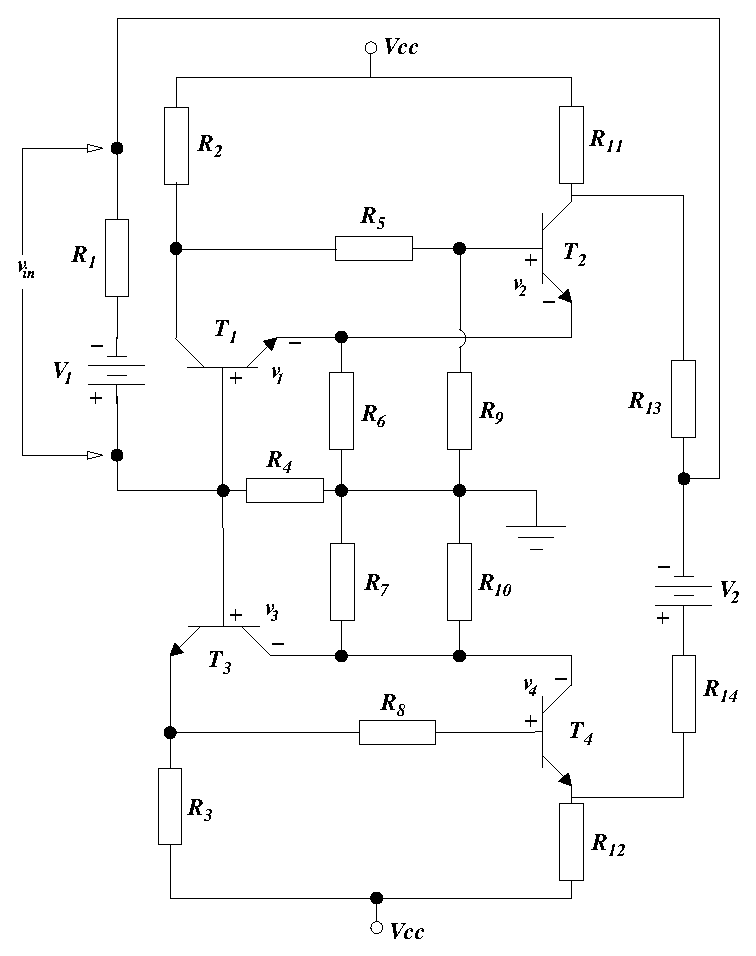
\includegraphics[scale=0.5]{nh3figs/chua.eps}}
\hspace{0.20in}
%% -- second subfigure ---
\subfloat[Half-sided Ebers-Moll model.]{
	\label{fig:subfig3:eber} 
	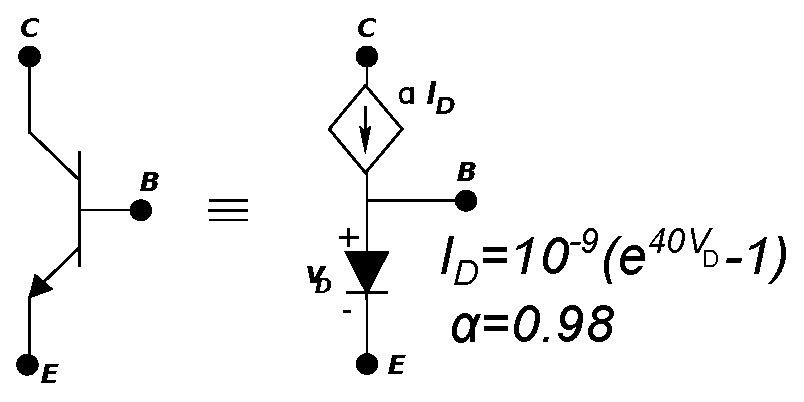
\includegraphics[scale=0.5]{nh3figs/eber.eps}}
\end{center}
\caption{Chua's circuit.}
\label{fig:subfig3}
\end{figure*}

The resulting equation system is:

{\tiny
\begin{equation}
\begin{array}{l}
f_1=4.3663v_2+0.6103168 \times 10^{-5} e^{(40v_1)}-12 \\ +0.2863168\times 10^{-5}e^{(40v_2)}=0 \\ \\
f_2=5.4v_1+v_3+0.3580\times 10^{-5}e^{(40v_1)}-22 \\+7\times 10^{-7}e^{(40v_3)}+  5\times 10^{-7}e^{(40v_4)}+0.6620\times 10^{-5}e^{(40v_2)}=0 \\ \\
f_3=4.3663v_4+0.6103168\times 10^{-5}e^{(40v_3)}-12 \\ +0.2863168\times 10^{-5}e^{(40v_4)}=0 \\
\end{array}
\end{equation}
}

Now, the DBH is applied to solve the circuit. The Homotopy formulation is expressed as:

{\tiny
\begin{displaymath}
\begin{array}{c}
H_1(f_1,\lambda)=\lambda(\lambda-1)(v_1-5)(v_1+5)-(\lambda-0.5)^2 f_1^2=0\\
H_2(f_2,\lambda)=\lambda(\lambda-1)(v_2-5)(v_2+5)-(\lambda-0.5)^2 f_2^2=0\\
H_3(f_3,\lambda)=\lambda(\lambda-1)(v_3-5)(v_3+5)-(\lambda-0.5)^2 f_3^2=0\\
H_4(f_4,\lambda)=\lambda(\lambda-1)(v_4-5)(v_4+5)-(\lambda-0.5)^2 f_4^2=0\\
\end{array}
\end{displaymath}
}
where bounding lines are $a=0$ and $b=1$, and the initial point for the Homotopy path is selected as $A=[v_1=-5.2,v_2=-5.2,v_3=-5.2,v_4=-5.2]$.

Equilibrium equation is the same as employed in \cite{homo_chua}. The variables to be solved are branch voltages: $v_1$, $v_2$, $v_3$ and $v_4$. Figure \ref{chuaf} shows the Homotopy path for branch voltage $v_1$. The final point for the path was $B=[v_1=-5.2,v_2=-5.2,v_3=5.2,v_4=-5.2]$. Finally, Homotopy was able to locate all the 9 solutions in just one path. 
This result is interesting considering that in recent works \cite{homo_yamamura}\cite{homo_jaewook} (applied to the same circuit) only one solution was found or some solutions were found by selecting (random or arbitrary) different initial points, that is, different and unconnected Homotopy paths. 


 Found solutions are:
{\tiny
\begin{displaymath}
\begin{array}{r}
\left[\begin{array}{r}
v_1 \\ v_2  \\ v_3  \\ v_4  \\
\end{array}\right]
\begin{array}{r}
 \\ = \\ \\ \end{array}
\underbrace{\left[\begin{array}{r}
-1.0510 \\ 0.3775 \\  0.3845\\  -3.9542 \\
\end{array}\right]}_{\mbox{Solution $S_1$}},
\underbrace{\left[\begin{array}{r}
-0.7119\\0.3775\\ 0.3350\\ 0.3653 \\ 
\end{array}\right]}_{\mbox{Solution $S_2$}},
\underbrace{\left[\begin{array}{r}
-0.5136\\0.3775\\-0.9682\\0.3775\\
\end{array}\right]}_{\mbox{Solution $S_3$}}, \\\\
\underbrace{\left[\begin{array}{r}
0.3242\\0.3703\\ -1.0395\\0.3775 \\
\end{array}\right]}_{\mbox{Solution $S_4$}},
\underbrace{\left[\begin{array}{r}
0.3300 \\ 0.3680 \\ 0.3367 \\ 0.3642 \\
\end{array}\right]}_{\mbox{Solution $S_5$}},
\underbrace{\left[\begin{array}{r}
0.3369\\ 0.3641\\0.3836\\-3.7069 \\
\end{array}\right]}_{\mbox{Solution $S_6$}},
\\\\
\underbrace{\left[\begin{array}{r}
0.3830 \\ -3.5446 \\ 0.3851 \\-4.0990 \\
\end{array}\right]}_{\mbox{Solution $S_7$}},
\underbrace{\left[\begin{array}{r}
0.3857\\ -4.2738\\ 0.3322\\0.3669
\end{array}\right]}_{\mbox{Solution $S_8$}},
\underbrace{\left[\begin{array}{r}
0.3869\\ -4.6321\\ -0.8002\\0.3775 \\
\end{array}\right]}_{\mbox{Solution $S_9$}}
\end{array}
\end{displaymath}}

\section{Conclusions}

A new kind of Homotopy was presented, it is named double bounded algebraic Homotopy, which contains just 2 solution lines. Also, various properties were demonstrated like the curvature radius at solutions and return points; here it was determined the influence of $C$ and $a$ on how acute the Homotopy path could be. Besides, it was demonstrated the symmetry of the Homotopy paths as well as the crossing point of the path through the symmetry axis. Additionally, it was illustrated the use of Homotopy in a mathematical and several circuital cases, showing its potential to be employed in analysis of non-linear circuits.


\begin{figure*}[hbtp]
\centering
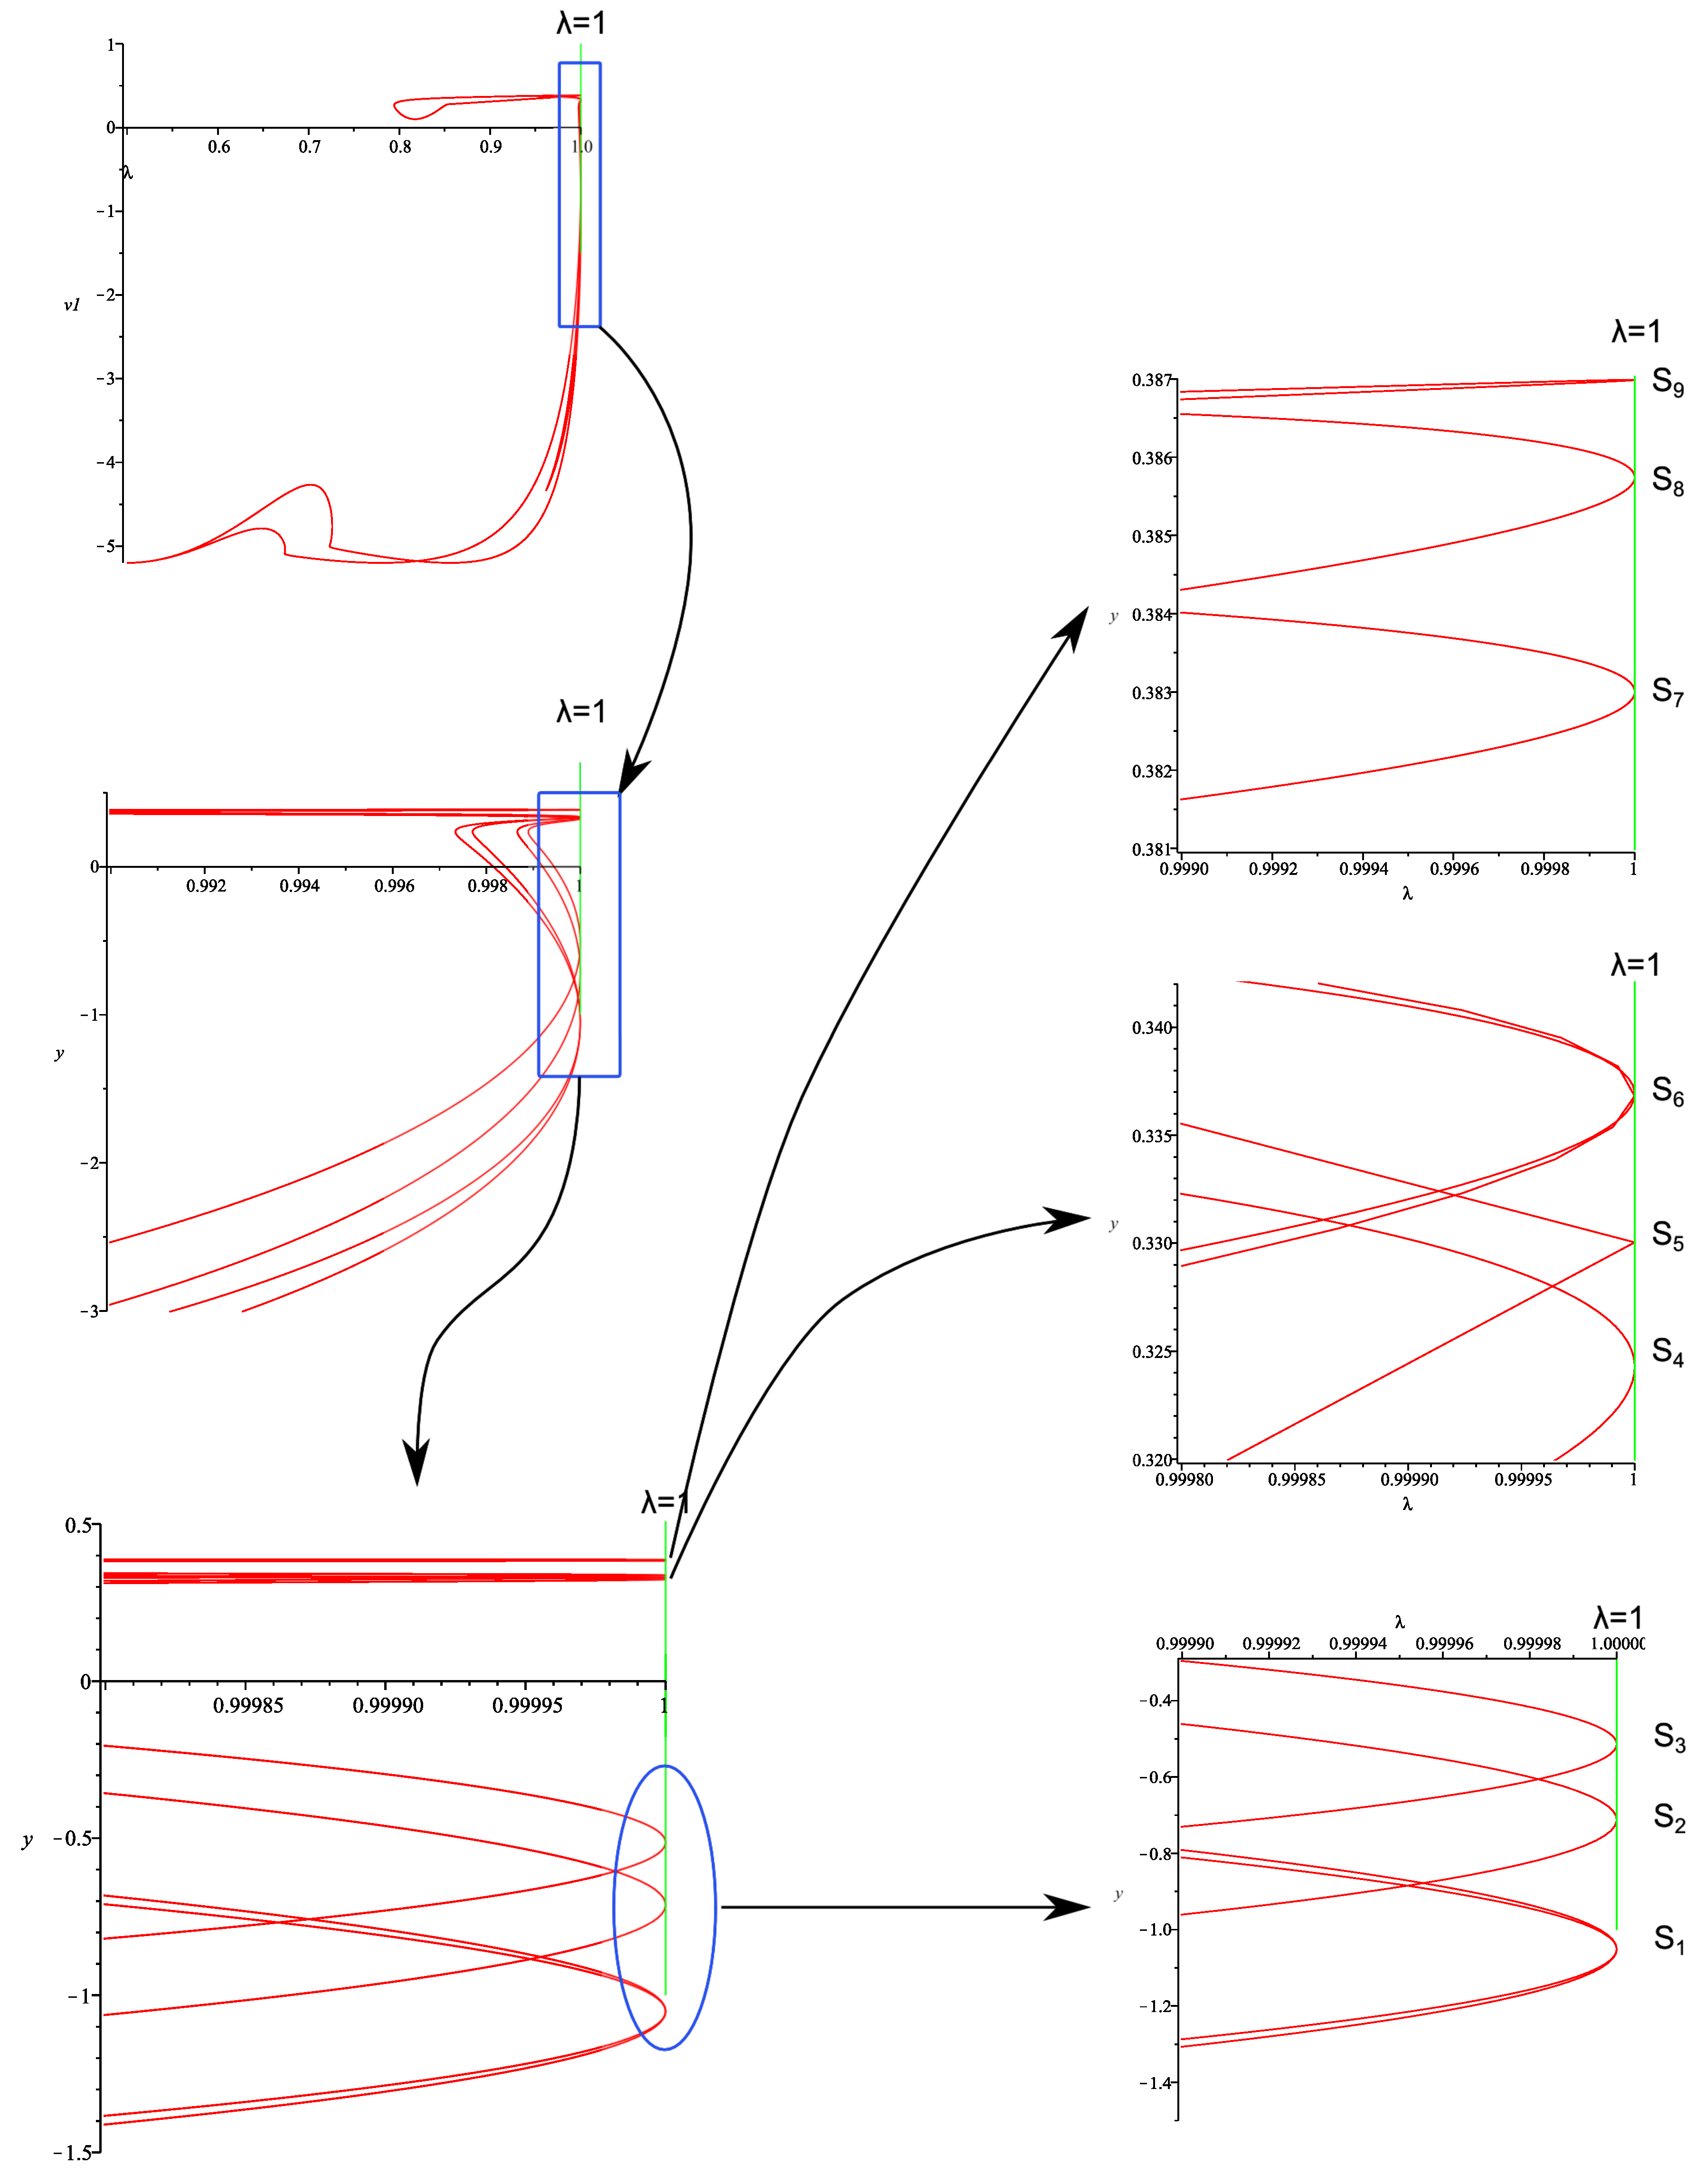
\includegraphics[scale=0.19]{nh3figs/chua_9sol_complete.eps}
\caption{Solutions for Chua's circuit.}
\label{chuaf}
\end{figure*}

\bibliographystyle{amsplain}
\bibliography{nuevah3_eng_2}

\end{document}
